% Options for packages loaded elsewhere
\PassOptionsToPackage{unicode}{hyperref}
\PassOptionsToPackage{hyphens}{url}
%
\documentclass[
  english,
  man,floatsintext]{apa6}
\usepackage{amsmath,amssymb}
\usepackage{lmodern}
\usepackage{ifxetex,ifluatex}
\ifnum 0\ifxetex 1\fi\ifluatex 1\fi=0 % if pdftex
  \usepackage[T1]{fontenc}
  \usepackage[utf8]{inputenc}
  \usepackage{textcomp} % provide euro and other symbols
\else % if luatex or xetex
  \usepackage{unicode-math}
  \defaultfontfeatures{Scale=MatchLowercase}
  \defaultfontfeatures[\rmfamily]{Ligatures=TeX,Scale=1}
\fi
% Use upquote if available, for straight quotes in verbatim environments
\IfFileExists{upquote.sty}{\usepackage{upquote}}{}
\IfFileExists{microtype.sty}{% use microtype if available
  \usepackage[]{microtype}
  \UseMicrotypeSet[protrusion]{basicmath} % disable protrusion for tt fonts
}{}
\makeatletter
\@ifundefined{KOMAClassName}{% if non-KOMA class
  \IfFileExists{parskip.sty}{%
    \usepackage{parskip}
  }{% else
    \setlength{\parindent}{0pt}
    \setlength{\parskip}{6pt plus 2pt minus 1pt}}
}{% if KOMA class
  \KOMAoptions{parskip=half}}
\makeatother
\usepackage{xcolor}
\IfFileExists{xurl.sty}{\usepackage{xurl}}{} % add URL line breaks if available
\IfFileExists{bookmark.sty}{\usepackage{bookmark}}{\usepackage{hyperref}}
\hypersetup{
  pdftitle={English Negative Constructions and Communicative Functions in Early Child Language},
  pdfauthor={Zoey Liu1 \& Masoud Jasbi2},
  pdflang={en-EN},
  pdfkeywords={negation; syntactic construction; communicative function; development; child language.},
  hidelinks,
  pdfcreator={LaTeX via pandoc}}
\urlstyle{same} % disable monospaced font for URLs
\usepackage{longtable,booktabs,array}
\usepackage{calc} % for calculating minipage widths
% Correct order of tables after \paragraph or \subparagraph
\usepackage{etoolbox}
\makeatletter
\patchcmd\longtable{\par}{\if@noskipsec\mbox{}\fi\par}{}{}
\makeatother
% Allow footnotes in longtable head/foot
\IfFileExists{footnotehyper.sty}{\usepackage{footnotehyper}}{\usepackage{footnote}}
\makesavenoteenv{longtable}
\usepackage{graphicx}
\makeatletter
\def\maxwidth{\ifdim\Gin@nat@width>\linewidth\linewidth\else\Gin@nat@width\fi}
\def\maxheight{\ifdim\Gin@nat@height>\textheight\textheight\else\Gin@nat@height\fi}
\makeatother
% Scale images if necessary, so that they will not overflow the page
% margins by default, and it is still possible to overwrite the defaults
% using explicit options in \includegraphics[width, height, ...]{}
\setkeys{Gin}{width=\maxwidth,height=\maxheight,keepaspectratio}
% Set default figure placement to htbp
\makeatletter
\def\fps@figure{htbp}
\makeatother
\setlength{\emergencystretch}{3em} % prevent overfull lines
\providecommand{\tightlist}{%
  \setlength{\itemsep}{0pt}\setlength{\parskip}{0pt}}
\setcounter{secnumdepth}{-\maxdimen} % remove section numbering
% Make \paragraph and \subparagraph free-standing
\ifx\paragraph\undefined\else
  \let\oldparagraph\paragraph
  \renewcommand{\paragraph}[1]{\oldparagraph{#1}\mbox{}}
\fi
\ifx\subparagraph\undefined\else
  \let\oldsubparagraph\subparagraph
  \renewcommand{\subparagraph}[1]{\oldsubparagraph{#1}\mbox{}}
\fi
% Manuscript styling
\usepackage{upgreek}
\captionsetup{font=singlespacing,justification=justified}

% Table formatting
\usepackage{longtable}
\usepackage{lscape}
% \usepackage[counterclockwise]{rotating}   % Landscape page setup for large tables
\usepackage{multirow}		% Table styling
\usepackage{tabularx}		% Control Column width
\usepackage[flushleft]{threeparttable}	% Allows for three part tables with a specified notes section
\usepackage{threeparttablex}            % Lets threeparttable work with longtable

% Create new environments so endfloat can handle them
% \newenvironment{ltable}
%   {\begin{landscape}\centering\begin{threeparttable}}
%   {\end{threeparttable}\end{landscape}}
\newenvironment{lltable}{\begin{landscape}\centering\begin{ThreePartTable}}{\end{ThreePartTable}\end{landscape}}

% Enables adjusting longtable caption width to table width
% Solution found at http://golatex.de/longtable-mit-caption-so-breit-wie-die-tabelle-t15767.html
\makeatletter
\newcommand\LastLTentrywidth{1em}
\newlength\longtablewidth
\setlength{\longtablewidth}{1in}
\newcommand{\getlongtablewidth}{\begingroup \ifcsname LT@\roman{LT@tables}\endcsname \global\longtablewidth=0pt \renewcommand{\LT@entry}[2]{\global\advance\longtablewidth by ##2\relax\gdef\LastLTentrywidth{##2}}\@nameuse{LT@\roman{LT@tables}} \fi \endgroup}

% \setlength{\parindent}{0.5in}
% \setlength{\parskip}{0pt plus 0pt minus 0pt}

% \usepackage{etoolbox}
\makeatletter
\patchcmd{\HyOrg@maketitle}
  {\section{\normalfont\normalsize\abstractname}}
  {\section*{\normalfont\normalsize\abstractname}}
  {}{\typeout{Failed to patch abstract.}}
\patchcmd{\HyOrg@maketitle}
  {\section{\protect\normalfont{\@title}}}
  {\section*{\protect\normalfont{\@title}}}
  {}{\typeout{Failed to patch title.}}
\makeatother
\shorttitle{Negation and communicative functions}
\keywords{negation; syntactic construction; communicative function; development; child language.
\newline\indent Word count: X}
\usepackage{lineno}

\linenumbers
\usepackage{csquotes}
\ifxetex
  % Load polyglossia as late as possible: uses bidi with RTL langages (e.g. Hebrew, Arabic)
  \usepackage{polyglossia}
  \setmainlanguage[]{english}
\else
  \usepackage[main=english]{babel}
% get rid of language-specific shorthands (see #6817):
\let\LanguageShortHands\languageshorthands
\def\languageshorthands#1{}
\fi
\ifluatex
  \usepackage{selnolig}  % disable illegal ligatures
\fi
\newlength{\cslhangindent}
\setlength{\cslhangindent}{1.5em}
\newlength{\csllabelwidth}
\setlength{\csllabelwidth}{3em}
\newenvironment{CSLReferences}[2] % #1 hanging-ident, #2 entry spacing
 {% don't indent paragraphs
  \setlength{\parindent}{0pt}
  % turn on hanging indent if param 1 is 1
  \ifodd #1 \everypar{\setlength{\hangindent}{\cslhangindent}}\ignorespaces\fi
  % set entry spacing
  \ifnum #2 > 0
  \setlength{\parskip}{#2\baselineskip}
  \fi
 }%
 {}
\usepackage{calc}
\newcommand{\CSLBlock}[1]{#1\hfill\break}
\newcommand{\CSLLeftMargin}[1]{\parbox[t]{\csllabelwidth}{#1}}
\newcommand{\CSLRightInline}[1]{\parbox[t]{\linewidth - \csllabelwidth}{#1}\break}
\newcommand{\CSLIndent}[1]{\hspace{\cslhangindent}#1}

\title{English Negative Constructions and Communicative Functions in Early Child Language}
\author{Zoey Liu\textsuperscript{1} \& Masoud Jasbi\textsuperscript{2}}
\date{}


\authornote{

Add complete departmental affiliations for each author here. Each new line herein must be indented, like this line.

Enter author note here.

Correspondence concerning this article should be addressed to Zoey Liu, . E-mail:

}

\affiliation{\vspace{0.5cm}\textsuperscript{1} Boston College\\\textsuperscript{2} UC Davis}

\abstract{
How does the abstract concept of linguistic negation develop in early child language? Prior research has suggested that abstract negation develops in stages and from more concrete communicative functions such as rejection, prohibition, or non-existence. The evidence for the emergence of these functions in stages is mixed, however, leaving the possibility that negation is an abstract concept since the beginning that can serve multiple specific functions depending on early communicative environment. Leveraging automatic annotations of large-scale child speech corpora in English, we examine the production trajectores of seven negative constructions that tend to convey communicative functions previously discussed in the literature. The results demonstrate the emergence and gradual increase of these constructions in child speech within the age range of 18-36 months. Production mostly remains stable, regular, and close to parents' levels after this age range. These findings are consistent with two hypotheses: first, that negation starts as an abstract concept that can convey multiple functions from the beginning; and second, that negation develops in distinct stages for separate communicative functions but the developmental patterns at different stages are early and quick, leaving our methods incapable of detecting them from the available corpus data.
}



\begin{document}
\maketitle

\hypertarget{introduction}{%
\section{Introduction}\label{introduction}}

\textcolor{blue}{(1) I made some changes in the abstract. Should we point out that the two hypothesis are (somewhat) contradicting? What satisfies as one starts earlier than another? Or would it be better ot say there's large overpa between the developmental patterns of negation conveying different communication functions.}

\textcolor{blue}{(2) I forgot whether the Introduction part is final. I made changes to the first paragraph, just trying to make it sound less like "English is special" :). I also feel perhaps in some places the term "child language" can be rephrased (child speech).}

\textcolor{blue}{(3) Is there a citation for *no* is one of the first produced words (but before that we said it's a morpheme) in English?}

Negation is a basic human concept and foundational to many areas of human knowledge such as logic and mathematics. Within the domain of linguistics, the abstract concept of negation is able to serve different communicative functions in different contexts. For example, in English, a coffee shop menu can combine the negative morpheme \emph{not} with the word ``coffee'' to form the expression of ``not coffee,'' which brings together diverse items such as tea and hot chocolate that are separate from just coffee. The same shop can use the other negative morphemes such as \emph{no} in a sign like ``no mask, no entry'' to regulate customer behavior. In Mandarin Chinese, an employee could say ``wo bu xihuan xingqiyi (''I not like Monday``),'' where \emph{bu} conveys negation to expressthe dislike of working on Mondays. Therefore, a fundamental question in cognitive development and language acquisition is: how does the concept of negation emerge and develop in the human mind.? In particular, are early developmental stages of negation in child speech specific to a few functions? Or does negation emerge as an abstract and multi-functional concept from the beginning?

Previous literature has proposed that abstract negation develops from less abstract communicative functions in fixed ordered stages (Bloom, 1970; Choi, 1988; McNeill \& McNeill, 1968; Pea, 1978). For instance, Darwin (1872) hypothesized that headshake as a sign for negation develops from infants' habit to refuse or reject food from parents by withdrawing their heads. Similarly, Pea (1978) proposed that at first, children use \emph{no} to convey ``rejection.'' In a second stage, they conceptualize and express non-existence of objects (e.g.~``no water {[}in the cup{]}''), and finally in the third stage, negation reaches an abstract status that can deny truth of statements (e.g.~``that is not a cow''). For Pea (1978), this order reflected a natural order in the conceptual space: from the more primitive concepts of internal desires to the more complex of external existence and finally abstract truth. As we will discuss in the next section, the theoretical and empirical landscape is, however, not so clean and simple. Over the past fifty years, many studies have proposed different communicative functions and orders of acquisition, without reaching a consensus. We will discuss some possible causes for this but it is important to emphasize previous literature has mainly argued for the following hypotheses: that the abstract concept of negation develops in fixed ordered stages from concrete communicative functions, and that children's early linguistic productions reflect these stages.

In this study, we provide evidence from child-speech corpora in English that suggests the functional development of negation in fixed ordered stages cannot be taken for granted. Given previous studies and our own, we conclude that it is possible that negation starts as an abstract concept that can be used to perform different communicative functions, and it is possible that it develops relatively quickly in functional stages becoming more abstract between 18-36 months of age.

In general discussion, we explain the limitations regarding inference from observational studies on children's linguistic productions. We argue that existence of stages in children's linguistic production does not necessarily imply stages in their conceptual or even linguistic development overall. Conversely, from absence of stages in children's linguistic productions one cannot conclude absence of stages in conceptual or linguistic development as a whole.

\hypertarget{previous-studies}{%
\section{Previous Studies}\label{previous-studies}}

\textcolor{blue}{ZL: (1) Is there a page number for the quoted content from Darwin? I also feel it's bit long}

\textcolor{blue}{ZL: (2) "Izanami had an abstract concept of negation"; What does this mean?}

Darwin (1872) proposed one of the earliest accounts that explained the emergence of negation based on its function. He hypothesized that negation originates from early expressions of human desire, and that nodding and shaking are the earliest expressions of affirmation and negation respectively. Darwin argued: ``With infants, the first act of denial consists in refusing food; and I repeatedly noticed with my own infants, that they did so by withdrawing their heads laterally from the breast, or from anything offered them in a spoon. In accepting food and taking it into their mouths, they incline their heads forwards \ldots{} {[}moreover{]} \ldots{} when the voice is exerted with closed teeth or lips, it produces the sound of the letter \emph{n} or \emph{m}. Hence we may account for the use of the particle \emph{ne} to signify negation, and possibly also of the Greek \emph{µn} in the same sense.'' In later research, this communicative function of negation was referred to as ``rejection'' or ``refusal.''

Unlike Darwin, McNeill and McNeill (1968) proposed a five-stage account for the conceptual development of negation that did not start with rejections. They studied the development of three Japanese negative morphemes (\emph{nai}, \emph{iya}, \emph{iiya}) in the speech of a 27-month-old Japanese speaking girl called Izanami. According to McNeill and McNeill (1968), in Japanese, \emph{nai} expresses falsity of statements (e.g.~``\emph{no} {[}that's not an apple{]}), \emph{iya} expresses desires (e.g.~''\emph{no} {[}I don't want an apple{]}``), and \emph{iiya} expresses contrast (e.g.~\emph{no} {[}I didn't have an apple. I had a pear{]}). Therefore their appearance in the speech of a child correspondingly reflects the developmental stages for the respective communicative functions. They reported that in the first stage, Izanami used a simple negation like \emph{nai} to express non-existence of events and objects. They also mentioned the early use of \emph{shira-nai} (''I don't know``) but did not incorporate it into their theoretical account. In the second stage, Izanami used negation to mark incorrectness of statements - similar to saying''false``. Such uses of negation were labeled as''denials" in later research. In stage three, negation was also used to express disapproval or rejection - similar to saying ``I don't want that.'' In the fourth stage, Izanami used negation to express contrasts - similar to saying ``not this but something else.'' Finally in the last stage, Izanami had an abstract concept of negation. These stages took about five months and started with expressing external states (non-existence of objects) before internal desires (rejection).

Bloom (1970) considered three communicative functions for early negation: non-existence, rejection, and denial. She studied three children, two from 19 months and another from 21 months of age. She argued that in all three children, negation was produced in the following order: non-existence, rejection, and denial. Table \ref{tab:bloom} provides a few examples for each category. Many of these examples do not immediately stand out as instances of their category. This is partly because many early examples are minimal and underspecified constructions that rely heavily on context for their interpretation. It is therefore hard to assess the intention behind the use of negation in such cases.

\begin{longtable}[]{@{}lll@{}}
\caption{\label{tab:bloom} Examples of non-existence, rejection, and denial negation in the speech of Eric, Kathryn, and Gia from Bloom (1970)}\tabularnewline
\toprule
Non-existence & Rejection & Denial \\
\midrule
\endfirsthead
\toprule
Non-existence & Rejection & Denial \\
\midrule
\endhead
no more choochoo train & no train & no Daddy hungry \\
no more noise & no want this & no more birdie \\
no children & no bear book & no ready \\
no it won't fit & no go outside & no tire \\
Kathryn no like celery & no dirty soap & no dirty \\
\bottomrule
\end{longtable}

\textcolor{blue}{ZL: "for about 90 minutes"; everyday?}

Pea (1978) studied six children between the ages of 8-24 months. Children were recorded monthly in their homes for about 90 minutes. All negative utterances (e.g.~containing \emph{no}, \emph{not}, \emph{all gone}, \emph{gone}, \emph{away}, \emph{stop}) and gestures (e..g headshakes and headnods) were annotated and analyzed. Pea (1978) reported that children first started by using negation to express internal states (i.e.~rejection), then external states (i.e.~disappearance), and finally they used negation to connect language and the external world, i.e.~truth-functional negation or denials). This was in direct contradiction to McNeill and McNeill (1968) who proposed that children start with expressing external states (non-existence) before internal states (rejection).

Villiers and Villiers (1979) studied the communicative functions of negation in the speech of Adam (27-31 months), Eve (18-22 months), and their own child Nicholas (23-29 months). The first two children were recorded for an hour every two or three weeks (Brown, 1973). They annotated children's examples of negation for six communicative functions: non-existence, disappearance, non-occurrence, cessation, rejection, and denial. Disappearance referred to cases where an object became hidden and cessation referred to the use of negation when a movement or action stopped (e.g.~``no walk'' when a toy stopped walking). They found rejections and denials to be the most frequent (and most reliable-to-annotate) functions of negation. Both functions were present from the earliest samples of children's speech and the authors concluded that there are individual differences in the functions of negation in child speech that mirror child-directed speech.

\textcolor{blue}{(1) wh "novel forms"?}

Choi (1988) looked at the speech of 11 children (2 English, 4 Korean and 5 French speaking) between 19 to 40 months of age. She reported 9 communicative functions for children's negation shown in Table \ref{tab:choi}. She matched each communicative function with linguistic forms and constructions that commonly convey it and proposed that these forms and functions develop in three phases. First, children used ``\emph{no}'' alone to express the four functions of nonexistence, prohibition, rejection, and failure. In the second phase, \emph{no} was used to express denial, inability, and epistemic negation. Novel forms such as ``\emph{not}+NP'' (e.g ``\emph{not a bee}''), \emph{can't} (e.g.~``\emph{I can't put back}''), and \emph{I don't know} were also used to express these functions. New forms emerged to distinguish the functions in the previous phase such as rejection as well (e.g.~``\emph{I don't want to}''). In the third phase, normative negation and inferential negation emerged in children's speech with modal auxiliaries like \emph{can't}. Negative forms for prohibition also emerged with the structure ``\emph{don't}+Verb.''

\begin{longtable}[]{@{}
  >{\raggedright\arraybackslash}p{(\columnwidth - 6\tabcolsep) * \real{0.28}}
  >{\raggedright\arraybackslash}p{(\columnwidth - 6\tabcolsep) * \real{0.34}}
  >{\raggedright\arraybackslash}p{(\columnwidth - 6\tabcolsep) * \real{0.14}}
  >{\raggedright\arraybackslash}p{(\columnwidth - 6\tabcolsep) * \real{0.24}}@{}}
\caption{\label{tab:choi} Examples of communicative functions and their forms in Choi (1988).}\tabularnewline
\toprule
Function & Definition & Forms & Example \\
\midrule
\endfirsthead
\toprule
Function & Definition & Forms & Example \\
\midrule
\endhead
Non-existence & expressing absence of entities & \emph{no}+V & ``\emph{no more}'' (after emptying a bag) \\
Failure & expressing absence of an event & \emph{it won't} & ``\emph{not work}'' (puzzle piece not fitting) \\
Prohibition & negating actions of others & \emph{don't} + V & \\
Rejection & negating the child's own actions & \emph{I don't want (to)} & \\
Denial & negating others' propositions & AUX + \emph{not} & ``\emph{no that's a pony}'' (in response to ``Is this a car?'') \\
Inability & expressing physical inability & & ``\emph{can't!}'' (taking two lego pieces apart) \\
Epistemic & lack of knowledge & \emph{I don't know} & ``\emph{I don't know}'' (in response to ``what color is this?'') \\
Normative & expressing expected norms & (you) \emph{can't} & ``\emph{Him can't go on a boat}'' \\
Inferential & child's inference about the listener & AUX + \emph{not} & ``\emph{I not broken this}'' (seeing a broken crayon) \\
\bottomrule
\end{longtable}

\textcolor{blue}{ZL: "for an hour" in total? Why leaving out "normative" and "inferential"?}

\textcolor{blue}{ZL: to put into quotes, or to not put into quotes? When to put into quotes? Formality consistency throughout manuscript}

Cameron-Faulkner, Lieven, and Theakston (2007) recorded a single English speaking child five times a week for an hour between the ages of 27 to 39 months. They classified his negative utterances into seven communicative functions by using categories from Choi (1988) and leaving out ``normative'' and ``inferential'' negation. They found examples of all seven functions in Brian's early speech. Starting at 27 months, single-word discourse-level \emph{no} was used to convey most functions but gradually other forms using \emph{not}, \emph{don't}, \emph{can't}, or \emph{won't} emerged and replaced \emph{no} in usage. For example with inability and prohibition, Brian mostly used \emph{no} and \emph{not} at 27 months but switched to \emph{can't} to express inability, and \emph{don't} to express prohibition at 39 months. Cameron-Faulkner, Lieven, and Theakston (2007) argued that at 27 months, Brian had a broad conceptualization of negation and likely represented it as a ``unitary category in conceptual space.''

\textcolor{blue}{ZL: functions in quotes}

In a recent study, Nordmeyer and Frank (2018) looked at twice-a-month recordings of five children between the 12-36 months of age (1-3 years) in the Providence corpus (Demuth, Culbertson, \& Alter, 2006) and classified children's negative utterances into seven functional categories: ``disappearance,'' ``prohibition,'' ``self-prohibition,'' ``rejection'' (refusal), ``failure,'' ``denial,'' and ``unfulfilled expectations.'' Self-prohibition referred to cases where children addressed a prohibition to themselves (e.g.~saying ``no'' to themselves when reaching for a forbidden object) and ``unfulfilled expectations'' referred to cases that expressed surprise when an object was not in an expected place, similar to some cases of non-existence in previous research. They found that refusals (rejections) and denials are the most common functions in children's productions and that children vary with respect to which function is produced first. In line with Villiers and Villiers (1979), they concluded that the developmental trajectory of different communicative functions of negation may not be as consistent across individuals as some previous research had suggested.

\begin{longtable}[]{@{}
  >{\raggedright\arraybackslash}p{(\columnwidth - 6\tabcolsep) * \real{0.11}}
  >{\raggedright\arraybackslash}p{(\columnwidth - 6\tabcolsep) * \real{0.13}}
  >{\raggedright\arraybackslash}p{(\columnwidth - 6\tabcolsep) * \real{0.18}}
  >{\raggedright\arraybackslash}p{(\columnwidth - 6\tabcolsep) * \real{0.58}}@{}}
\caption{\label{tab:summary} Summary of previous studies on the development of negation's communicative functions.}\tabularnewline
\toprule
Study & Number of Children & Age Range (Months) & Proposed Functional Stages \\
\midrule
\endfirsthead
\toprule
Study & Number of Children & Age Range (Months) & Proposed Functional Stages \\
\midrule
\endhead
McNeill and McNeill (1968) & 1 & 27-32 Months & non-existence \textgreater{} denial (non-contrastive) \textgreater{} rejection \textgreater{} denial (contrastive) \\
Bloom (1970) & 3 & 19-28 Months & non-existence \textgreater{} rejection \textgreater{} denial \\
Pea (1978) & 6 & 8-24 & rejection \textgreater{} non-existence \textgreater{} denial \\
Villiers and Villiers (1979) & 3 & 18-31 & rejection, denial (variable) \\
Choi (1988) & 11 & 19-40 & nonexistence, prohibition, rejection, failure \textgreater{} denial, inability, epistemic \textgreater{} normative, inferential \\
Cameron-Faulkner, Lieven, and Theakston (2007) & 1 & 27-39 & non-existence, failure, prohibition, rejection, denial, inability, epistemic \\
Nordmeyer and Frank (2018) & 5 & 12-36 & denial, rejection, prohibition, failure, disappearance (variable) \\
\bottomrule
\end{longtable}

Table \ref{tab:summary} provides a summary of previous research on the communicative functions of negation in children's speech. As the summary shows, there is currently no consensus on which functional categories should be included or in which order they are produced. Here we are going to discuss three possible reasons for this lack of consensus. First, Villiers and Villiers (1979) and Nordmeyer and Frank (2018) have emphasized that there is considerable variability among children and their parents in their use of negation. Given that previous studies have typically considered only a few children (3-4 on average), they could have reached conclusions that are true of their sample but not of the population of English-speaking children. Second, previous studies have used monthly or fortnightly recordings of children's speech for about 60-90 minutes per recording session. Given that children produce many hours of speech daily, such sparse sampling may have created accidental gaps for certain communicative functions and consequently made it as if functions appear in ordered stages. The only study with relatively dense recording is Cameron-Faulkner, Lieven, and Theakston (2007) which reports the presence of all communicative functions in the child's speech from early on. The only caveat to this study is that recordings start at a later age than many other studies.

Third, previous research shows that defining and detecting the communicative functions of negation is not a trivial task. Different studies have sometimes used different basic categories and different definitions or criteria for classifying negative utterances. Therefore, what counts as an instance of rejection or non-existence may vary among studies and contribute to the reported variability. Most importantly, annotations focus on many underspecified utterances such as ``\emph{no car}'' or ``\emph{no more}'' which are highly ambiguous and can count as an instance of different communicative functions. Does \emph{no car} mean ``there is no car here'' or ``I don't want a toy car?'' Researchers often have to rely on the context but the context is not fully represented in many child language corpora used for annotations. More importantly, this approach is not scalable to larger numbers of children and bigger corpora since manual annotations take considerable amount of time, energy, and training. In the next section, we discuss how the current study addresses these three issues.

\hypertarget{current-study}{%
\section{Current Study}\label{current-study}}

We build on previous research and address the methodological issues discussed in previous section in two ways. First, in this study we use large corpora of parent-child interactions, aggregating speech samples from X children between the ages of 1-6 years (12-72 months). If the lack of consensus in previous research was mainly due to the small number of children studied, increasing this number should address the issue. Aggregating speech samples across children would also provide denser samples at each time interval and reduce the possibility of accidental gaps in a supposed stage. The reasoning behind this approach is that despite individual variation, if there are major developmental stages in children's production of negation that hold on average across children, these stages should be detectable in such large aggregate corpus of child speech.

Second, in this study we shift the focus from detecting and classifying negative communicative functions such as rejection to detecting and classifying negative constructions that typically communicate them. Here by negative constructions, we refer to syntactic constructions modified by any one of the three negative morphemes in English: \emph{no}, \emph{not}, \emph{n't}. Table \ref{tab:constructions} summarizes the constructions and communicative functions used in this study.

This approach has several advantages. To begin with, negative constructions are more concrete and easier to define and classify. This way we can avoid inconsistent definitions and criteria for classification across different studies. For example, utterances that combine negation with the main verb \emph{want} (e.g.~``\emph{I don't want that}'') constitute a construction that typically conveys rejection. In addition, due to their concrete definitions, constructions can be detected and classified automatically in large corpora. While it is difficult to manually annotate for examples of rejection across thousands of utterances, it is relatively easier to automatically detect utterances containing the verb \emph{want} modified by negative morphemes. This approach is similar in spirit to that of Choi (1988) who manually annotated for both communicative functions and their common linguistic forms (Table \ref{tab:summary}).

\textcolor{blue}{(1) "produce shorter forms before longer ones"; Possible Citation?}

\textcolor{blue}{(2) I did not understand "will probably estimate an upper bound on when..."}

\textcolor{blue}{(3) I'm a little hesitant to call it "response particle"; there's debate over whether particle is a thing; I'd be leaning towards "discourse response marker"}

One downside of focusing on negative constructions is that it may systematically underestimate children's knowledge of negation. Due to early limited productive capacities, children produce shorter forms before longer ones. Therefore, they can convey a communicative function like rejection using a simple \emph{no} before they can produce the full construction ``\emph{I don't want that}.'' Focusing on children's production of explicit constructions, we will probably estimate an upper bound on when children can convey a communicative function. To make up for this, besides investigating negative constructions at the sentence level, we also investigate children and parents' use of \emph{no} as a response particle at the discourse level. Negative discourse particles like \emph{no} can be used in isolation to negate the content of a previous utterance. For example, if a mother asks ``do you want some milk?'' and the child responds with ``no,'' the negative particle anaphorically targets the proposition ``I want some milk'' and negates it: ``I don't want milk.'' By using negative discourse particles like \emph{no}, children can convey complex negative content without actually producing them in words. This approach is useful early in their development when they have limited productive capacities. In our analyses, we also look at children and parents' use of negative discourse particles. More specifically, we examine the constructions in the immediate previous utterance in the discourse that are negated by these particles. The analyses of these constructions in the preceding utterance can capture communicative functions that the response particle \emph{no} conveys before children are capable of producing their full syntactic forms.

\begin{table*}[h]
\small
\centering
\begin{tabular}{rrr}
\hline
\textbf{Function} & \textbf{Negative morpheme combines with} & \textbf{Negative Examples} \\
\hline
Rejection & *like*/*want* & *I not like it*; *not want it* \\
Non-existence & *there*-expletive & *there is no soup*  \\
Prohibition & imperative subjectless *do* & *do not spill milk* \\
Inability & *can* & *I cannot zip it*  \\
Labeling (Denial) & nominal/adjectival predicates & *that's not a crocodile*; *it's no interesting  \\
Epistemic & *know*/*think*/*remember*  & *I not know/think/remember*  \\
Possession & *have*/possesive pronouns & *not have the toy*; *not mine*  \\
\hline
\end{tabular}
\caption{English negative communicative functions and constructions used in this study.}
\end{table*}

Table: \label{tab:constructions} Negative constructions used in this study that typically convey communicative functions studied in previous functional accounts of negation development

\hypertarget{data-and-preprocessing}{%
\subsection{Data and preprocessing}\label{data-and-preprocessing}}

For child speech data in English, we turned to the CHILDES database (MacWhinney, 2000)\footnote{Code and data are in quarantine at \url{https://github.com/zoeyliu18/Negative_Constructions.}} and selected English speaking children with typical development within the age range of 12-72 months. Parents' and children's utterances were extracted via the childes-db (Sanchez et al., 2019) interface using the programming language R. In order to obtain (morpho)syntactic representations for parents' and children's utterances, we used the dependency grammar framework (Tesnière, 1959). Part-of-speech (POS) tags for each token within an utterance were automatically derived using Stanza (Qi, Zhang, Zhang, Bolton, \& Manning, 2020), an open-source natural language processing library; dependency relations for all utterances were acquired also in an automatic fashion using DiaParser (Attardi, Sartiano, \& Yu, n.d.), a dependency parsing system that has been demonstrated to achieve excellent performance for at least written texts in English.

\textcolor{blue}{(1) In the following paragraph, there's duplicated content with the previous section. I'm wondering if we should remove it here.}

\textcolor{blue}{(2) I changed "test children's knowledge" to "test children's production"}

\textcolor{blue}{(3) I like the last sentence of the following paragrah; Perhaps we could move it to the end of the last paragrah in the previous section; and maybe add the word "possibly", since it's not completely sure children understand them.}

We focus on seven negative constructions shown in Table 1 that tend to convey the communicative functions of rejection, non-existence, prohibition, inability, labeling, epistemic state, and possession. We test children's production of these constructions at two levels: sentence level and discourse level. Negation is marked in two fundamentally different ways in English and many other languages. First, at sentence level, morphemes such as \emph{no}, \emph{not}, or the reduced form \emph{n't} combine with other lexical items to form a negative sentence. For example in sentence level rejection, \emph{n't} can combine with \emph{want} to form ``\emph{I don't want to go}.'' Second, negative response particles such as \emph{no} can be used anaphorically to negate a previous utterance in discourse. For example in discourse level rejection, when a parent asks ``\emph{Do you want to go?}'' a child can respond with \emph{No!}. Here, the negative discourse particle stands for the proposition ``I don't want to go.'' Children's earliest negative productions are dominated by discourse level negation, presumably because it is shorter and easier to produce when children are limited in their productive capacity. Nevertheless, successful communication with discourse level negation can indicate the children understand the propositions conveyed it.

At the sentence level, we characterized the syntactic features of the negative utterances associated with each communicative function, then classified utterances based on these features in a rule-based fashion with the help of POS information and syntactic dependencies. To decouple the development of the syntactic construction from the development of negation in that construction, we also examined the production of positive counterparts to each negative construction. The positive counterpart of our negative constructions share the same syntactic features (e.g.~same head verb) but they have no negative morphemes. These positive constructions do not express the same communicative function as their negative counterparts. Our main purpose for including the positive counterparts is to factor in the development of the syntactic construction without negation.

\textcolor{blue}{ZL: cases like *no no no*}

At the discourse level, we need to analyze the negative constructions that the discourse particle \emph{no} stands for. To achieve this, we selected utterances that started with negative discourse particles like ``no no I like it.'' These instances were tagged with the dependency relation ``discourse'' by our dependency parser. For each negative utterance identified this way, we extracted the previous utterance (the antecedent) in the discourse context. For child speech, we included interactions (negative utterances + their antecedents) where antecedents were produced by either the parents or the children themselves. For parent speech, we only included interactions where the antecedent was produced by children. We then applied the same analyses performed to sentence level constructions to these antecedent utterances. The assumption here is that the negative discourse particles are implicitly negating the content of their discourse antecedents.

\textcolor{blue}{(1) changed "moving ratio" to "cumulative ratio"}

\textcolor{blue}{(2) log ratio to ratio}

\textcolor{blue}{(3) equation (2) changed; double check}

\textcolor{blue}{(4) in some plots, the cumulative ratio is supposed to start below ratio, unless I'm not understanding the original issue}

\hypertarget{measures}{%
\subsection{Measures}\label{measures}}

We took age as a proxy for children's development and divided the 12-72 months range into monthly bins. We used the following two metrics for each age bin and communicative function. First, we defined the ratio \(R_{c,i}\) for construction \(c\) and age bin \(i\) as the number of utterances in construction \(c\) and age bin \(i\) divided by the total number of utterances produced at age bin \(i\). For example at age 30 months, children produced a total of 81,302 utterances, out of which 391 were classified as rejections. Therefore the ratio of rejection at 30 months is 391/81,302 = 0.005.

\(R_{c, i} = \frac{\#U_{c,i}}{\#U_{i}}\)

Second, we borrowed the measure of ``cumulative (moving) ratio'' from the analysis of time series data (Wei, 2006). We defined the cumulative ratio \(CR_{c,i}\) for a construction \(c\) at age bin \(i\), as the sum of the number of utterances produced with construction \(c\) from the first age bin to age bin \(i\), divided by the sum of all utterances produced between the first age bin and age bin \(i\). For example up to age 30 months, children in our corpus produced 721,748 total utterances, out of which 2,166 were instances of rejection. Therefore, the cumulative ratio of rejection at age 30 months is 2,166/721,748 = 0.003. The cumulative ratio has the advantage that at each age bin, it takes into account the productions in previous age bins. Assuming that children accumulate linguistic knowledge throughout their development, this measure provides a more realistic and stable measure of children's productive capacity at each age.

\(CR_{c, i} = \frac{\sum_{n=1}^{i} \#U_{c,n}}{\sum_{n=1}^{i} \#U_{n}}\)

The two ratios mentioned above were calculated for negative constructions and their positive counterparts at sentence and discourse levels for children as well as parents. In this study we use parents' speech as a benchmark for children's development. Therefore, our figures show children's productions side by side the production of parents at the corresponding age of children. In what follows, we describe in detail the results for each communicative function and its associated negative constructions.

\hypertarget{negative-constructions}{%
\subsection{Negative Constructions}\label{negative-constructions}}

\hypertarget{rejection}{%
\subsubsection{Rejection}\label{rejection}}

For instances of ``rejection'' and positive counterparts, we selected utterances in which the lemma of the head verb of the phrase is either \emph{like} or \emph{want}. For negative instances, the head verb is modified by one of the three negative morphemes \emph{no}, \emph{not} or \emph{n't}, whereas cases including the same head verb but without negation were classified as positive. Table \ref{tab:rejection} shows examples of negative utterances including those in which the speakers describe their own desires with or without an auxiliary verb (e.g.~1 and 2), as well as cases that express rhetorical inquiries of desires from one interlocutor to another (e.g.~3), and instances where the speaker is describing the desires of somebody else (e.g.~4). We classified a total of 20,641 negative utterances (child: 9,398; parent: 11,243), and a total of 180,881 negative utterances (child: 63,427; parent: 117,454).

\begin{longtable}[]{@{}ll@{}}
\caption{\label{tab:rejection} Examples of sentence-level rejection (negative) and positive counterparts in children's speech.}\tabularnewline
\toprule
Rejection (Negative) & Positive Counterpart \\
\midrule
\endfirsthead
\toprule
Rejection (Negative) & Positive Counterpart \\
\midrule
\endhead
\emph{I no like sea} & \emph{she likes cheese} \\
\emph{don't wanna go} & \emph{I want it} \\
\emph{don't you wanna try it} & \emph{I wanna have that} \\
\emph{Sarah doesn't like that either} & \emph{she likes this one} \\
\bottomrule
\end{longtable}

\begin{figure}[H]

{\centering 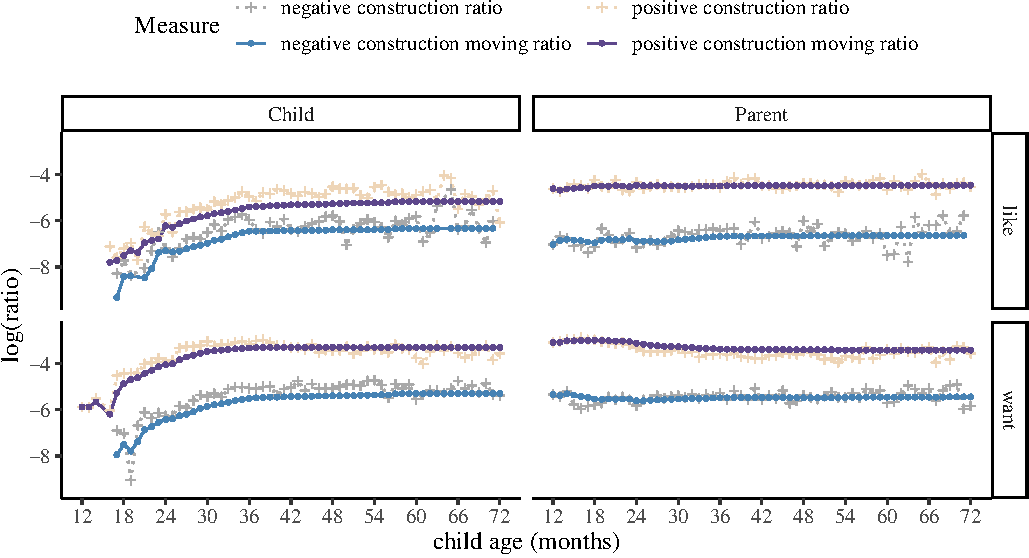
\includegraphics{neg_construction_article_files/figure-latex/emotion-1} 

}

\caption{Ratios and cumulative ratios for the production of rejection at the sentence level for children between 12 to 72 months of age, and their parents.}\label{fig:emotion}
\end{figure}

\begin{figure}[H]

{\centering 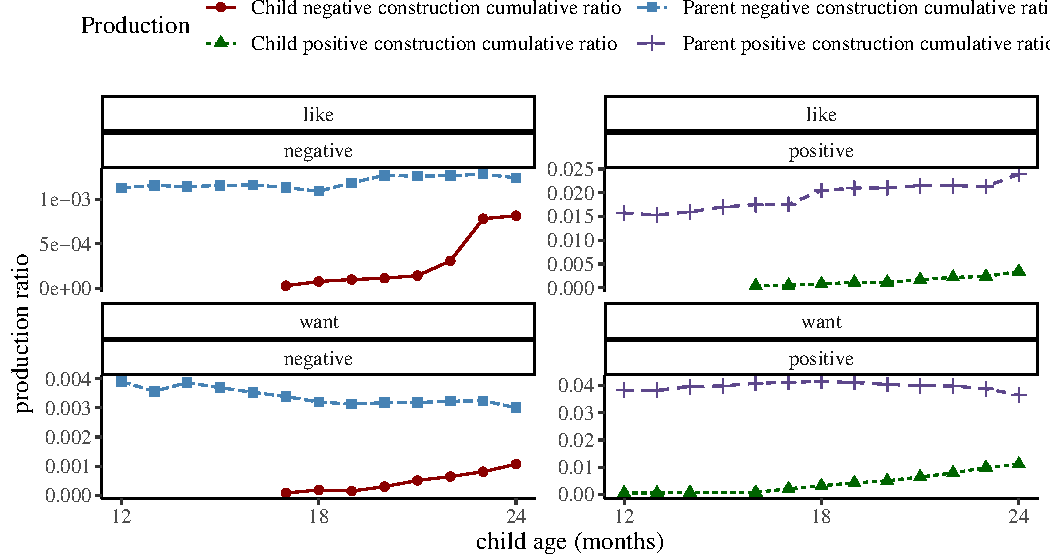
\includegraphics{neg_construction_article_files/figure-latex/emotionbegin-1} 

}

\caption{Ratios and cumulative ratios for the production of rejection at the sentence level for children between 12 to 24 months of age, and their parents}\label{fig:emotionbegin}
\end{figure}

Starting with our analysis at the sentence level, Figure \ref{fig:emotion} shows the ratios and cumulative ratios of parents' and children's instances of rejection and positive counterparts on a logarithmic scale (y-axis) with age along the x-axis. Overall, we see a similar pattern of production for rejection whether the head verb is \emph{want} or \emph{like}. Comparing the cumulative ratios between parents and children, children's production of rejection gradually increases between the ages of 18 and 30 months. After about 30 months of age, children's production of these constructions stays at a relatively constant rate and close to parent levels. In all age bins, the production ratio for negative utterances is lower than that for their positive counterparts.

On the discourse level, we investigated discourse interactions (antecedent + negative utterance) in which the antecedent had one of the head verbs \emph{like} or \emph{want}, yet the head verb did not have to be modified by negative morphemes. Table \ref{tab:disreject} shows a few examples. We found a total of 11,021 such utterances (child: 7,903; parent: 3,118). As shown in Figure 2, children's production of negation as discourse response variables increases regularly from the age of 24 - 36 months\footnote{For each communicative function, at the discourse level we also examined cases of different subtypes (e.g. different head verbs) separately; though due to data sparsity issues, we collapsed these instances for our final analyses}. Overall negative morphemes are applied at the discourse level more frequently in child speech compared to parent speech.

\begin{longtable}[]{@{}ll@{}}
\caption{\label{tab:disreject} Examples of discourse-level rejections and their antecedents in parents' and children's speech.}\tabularnewline
\toprule
Antecedent & Utterance \\
\midrule
\endfirsthead
\toprule
Antecedent & Utterance \\
\midrule
\endhead
Parent: \emph{I want you to try it} & Child: \emph{no no no} \\
Parent: \emph{would you like to go} & Child: \emph{no no} \\
Child: \emph{I don't like that} & Parent: \emph{no honey you have to try it} \\
Child: \emph{I want it} & Parent: \emph{no this is not for you} \\
\bottomrule
\end{longtable}

\begin{figure}[H]

{\centering 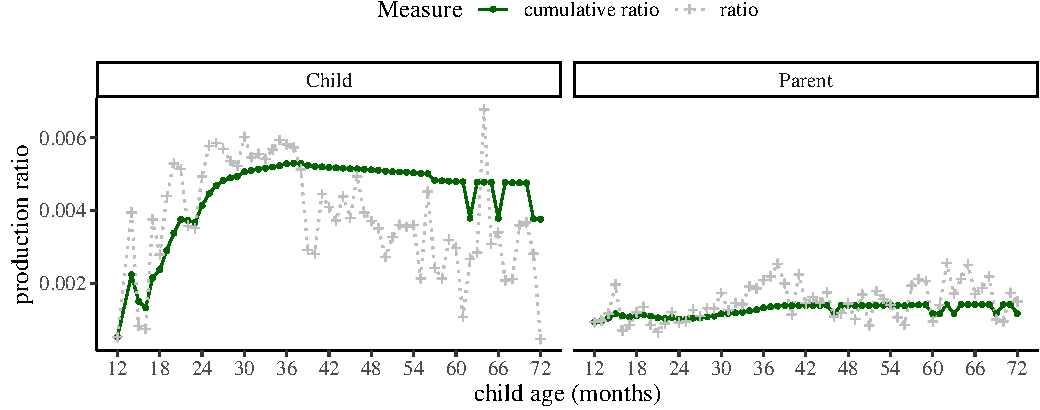
\includegraphics{neg_construction_article_files/figure-latex/emotiondiscourse-1} 

}

\caption{Ratios and cumulative ratios for the production of rejection at the discourse level for children between 12 to 72 months of age, and their parents.}\label{fig:emotiondiscourse}
\end{figure}

\begin{figure}[H]

{\centering 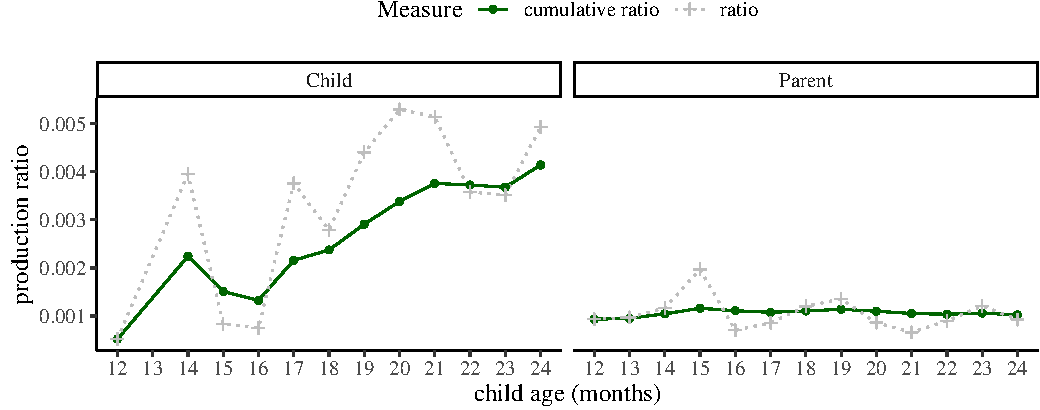
\includegraphics{neg_construction_article_files/figure-latex/emotiondiscoursebegin-1} 

}

\caption{Ratios and cumulative ratios for the production of rejection at the discourse level for children between 12 to 24 months of age, and their parents.}\label{fig:emotiondiscoursebegin}
\end{figure}

\hypertarget{non-existence}{%
\subsubsection{Non-existence}\label{non-existence}}

For this function we searched for the English existential construction and extracted utterances that had \emph{there}-expletives, followed by a copula, and a noun phrase (phrases headed by either nouns or pronouns). We classified utterances where the predicate was modified by negation as negative, and the rest as positive. This led to a total of 1,983 negative utterances (child: 498; parent: 1,485), and a total of 35,287 positive utterances (child: 8,385; parent: 26,902).

\begin{longtable}[]{@{}ll@{}}
\caption{\label{tab:nonexist} Examples of sentence-level non-existence (negative) and positive counterparts in children's speech.}\tabularnewline
\toprule
Non-existence (Negative) & Existentials (Positive) \\
\midrule
\endfirsthead
\toprule
Non-existence (Negative) & Existentials (Positive) \\
\midrule
\endhead
\emph{there's no (more) water} & \emph{there are books} \\
\emph{there isn't it} & \emph{there is it} \\
\bottomrule
\end{longtable}

At the sentence level, children produced negative constructions to express non-existence less frequently than the positive counterparts. As Figure \ref{fig:existence} shows, the cumulative ratio for the production of non-existence increases from 18 to 36 months. Around and after 36 months of age, children's productions reaches a stable cumulative ratio close to that of adults. Notice that there appears to be fluctuations of cumulative ratios between the age of 19 and 25 months in child production. A closer inspection of the data reveals that within that age range, the frequency of negative utterances at most ages is either one or zero. Therefore while the number of total utterances increases along the developmental trajectory, the cumulative ratio for negative utterances actually decreases.

\begin{figure}[H]

{\centering 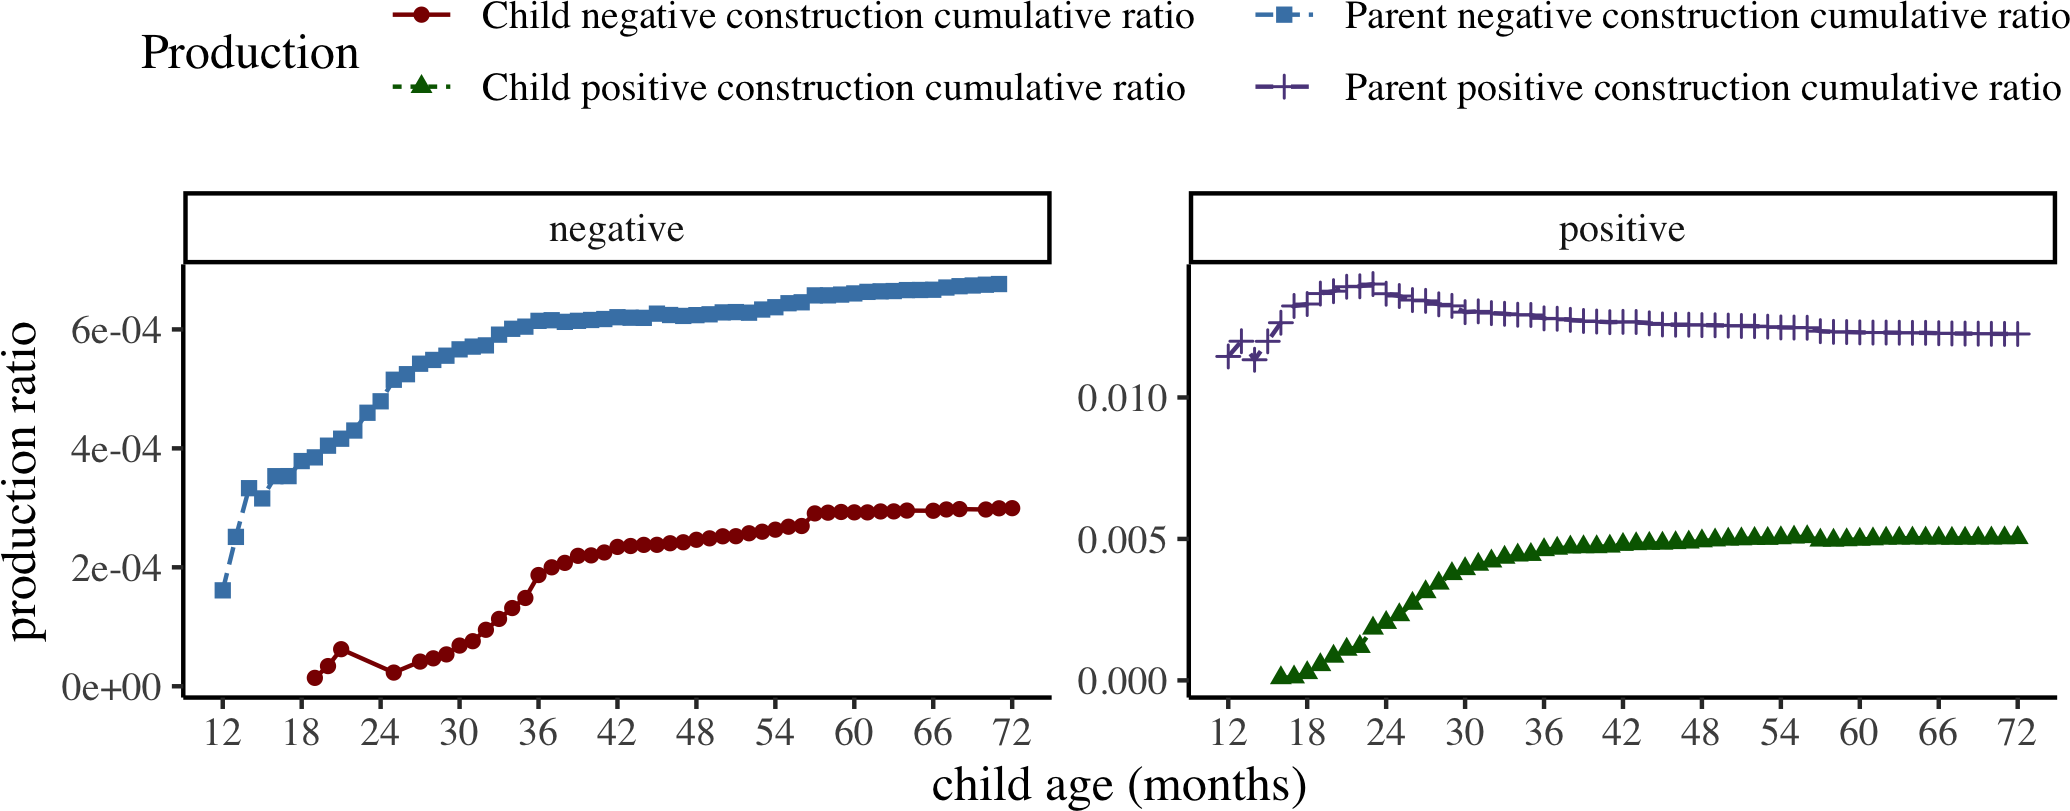
\includegraphics{neg_construction_article_files/figure-latex/existence-1} 

}

\caption{Ratios and cumulative ratios for the production of non-existence at the sentence level for children between 12 to 72 months of age, and their parents.}\label{fig:existence}
\end{figure}

\begin{figure}[H]

{\centering 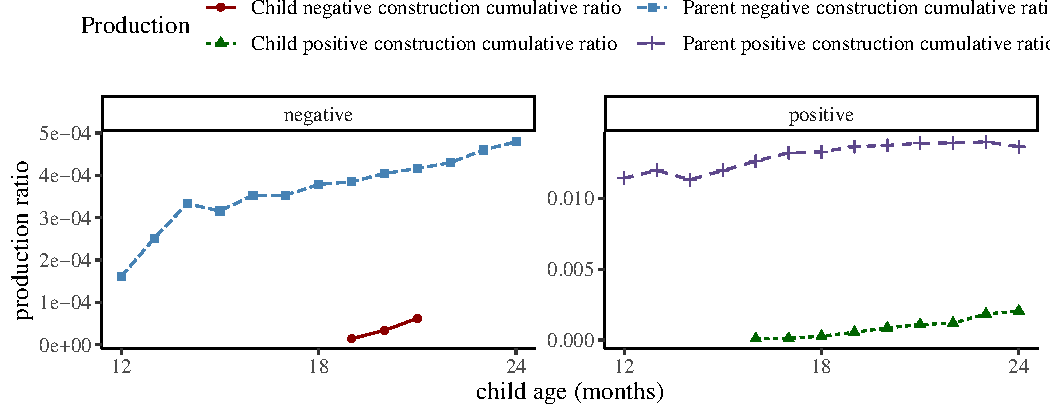
\includegraphics{neg_construction_article_files/figure-latex/existencebegin-1} 

}

\caption{Ratios and cumulative ratios for the production of non-existence at the sentence level for children between 12 to 24 months of age, and their parents.}\label{fig:existencebegin}
\end{figure}

For non-existence at the discourse level, we applied similar selection criteria and extracted negative utterances with existential constructions in their antecedents (Table \ref{tab:disexist}). This led to a total of 1,202 utterances (child: 828; parent: 374). As Figure \ref{fig:exstencediscourse} shows, we could find an increase in children's responses with \emph{no} to parents' existential utterances between the ages of 18 and 36 months. After 36 months, despite the fact that ratios show considerable fluctuations, the cumulative ratios of parents and children seem stable and similar. Therefore with non-existence, both sentence level and discourse level analyses point to substantial development in the age rage of 18-36 months.

\begin{longtable}[]{@{}ll@{}}
\caption{\label{tab:disexist} Examples of discourse-level non-existence and their antecedents in parents' and children's speech.}\tabularnewline
\toprule
Antecedent & Utterance \\
\midrule
\endfirsthead
\toprule
Antecedent & Utterance \\
\midrule
\endhead
Parent: \emph{is there a bunny} & Child: \emph{no no bunny} \\
Child: \emph{there is my ball} & Parent: \emph{no that's not yours} \\
\bottomrule
\end{longtable}

\begin{figure}[H]

{\centering 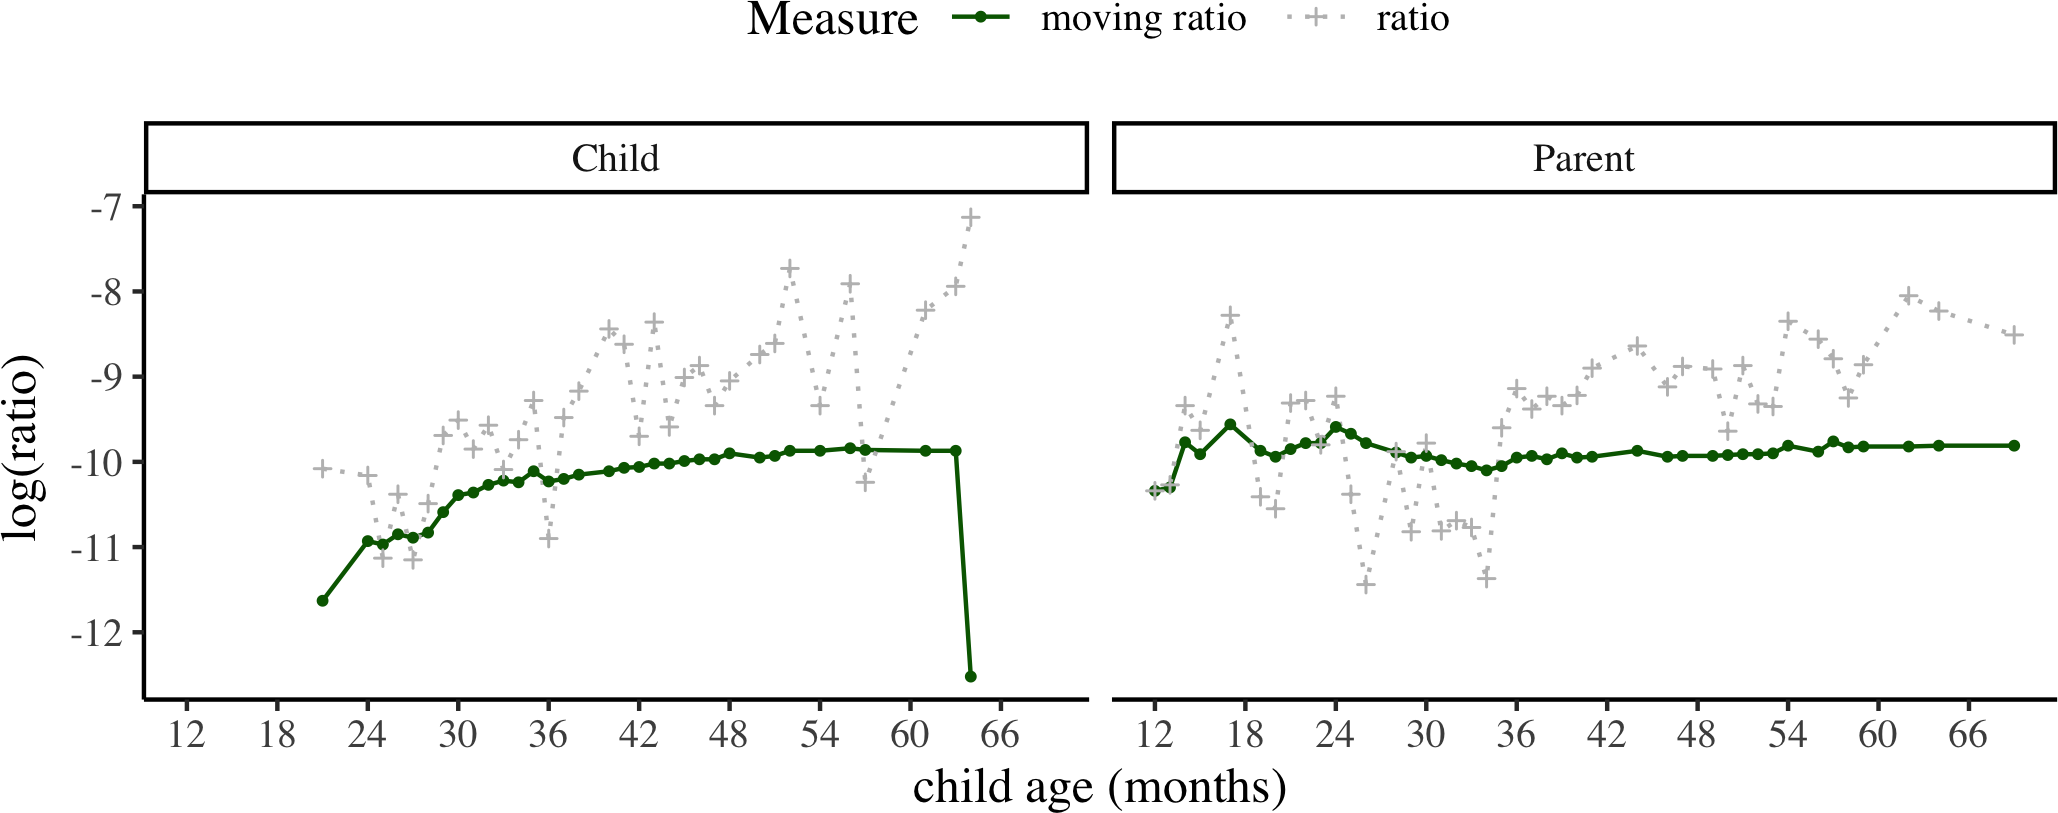
\includegraphics{neg_construction_article_files/figure-latex/existencediscourse-1} 

}

\caption{Ratios and cumulative ratios for the production of non-existence at the discourse level for children between 12 to 72 months of age, and their parents.}\label{fig:existencediscourse}
\end{figure}

\begin{figure}[H]

{\centering 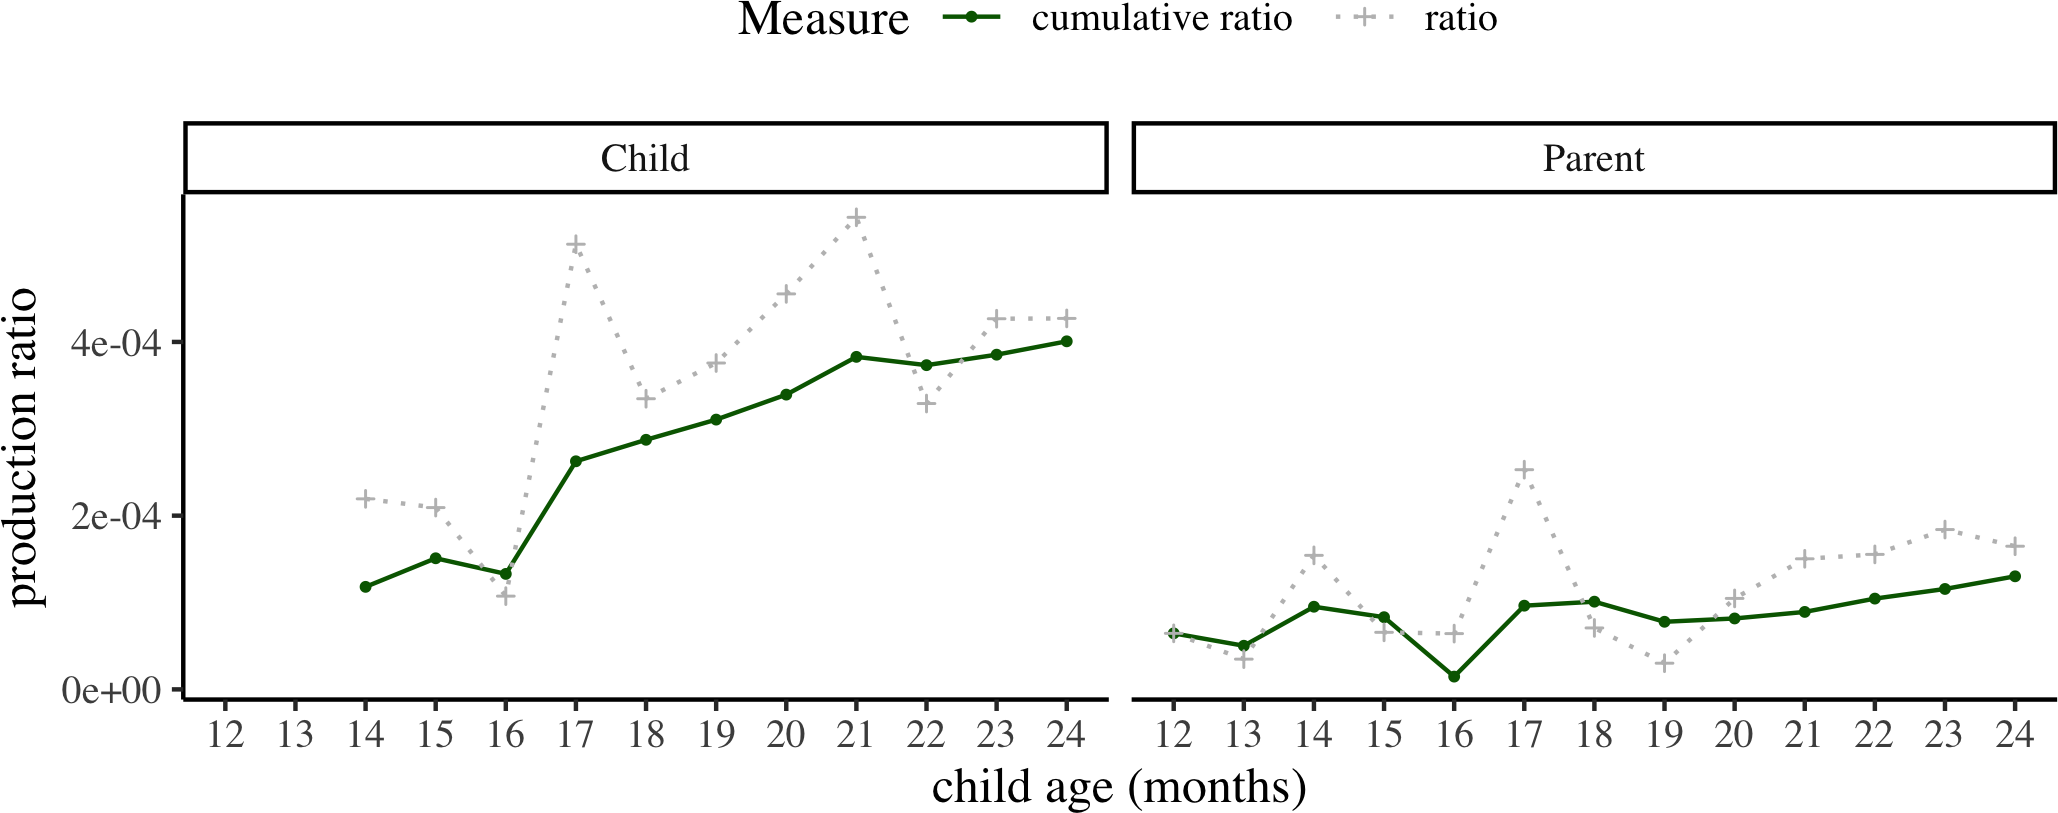
\includegraphics{neg_construction_article_files/figure-latex/existencediscoursebegin-1} 

}

\caption{Ratios and cumulative ratios for the production of non-existence at the discourse level for children between 12 to 24 months of age, and their parents.}\label{fig:existencediscoursebegin}
\end{figure}

\hypertarget{prohibition}{%
\subsubsection{Prohibition}\label{prohibition}}

For constructions that typically convey prohibition, we extracted utterances that were annotated as imperatives in CHILDES. In particular, we selected instances where the head verbs do not take any subjects. As before, cases without any negative morphemes are considered as positive. For negative constructions, we chose structures where the negative morphemes are combined with the auxiliary verb \emph{do} (\emph{do}, \emph{does}, \emph{did}) and they together modify the head verbs of the sentences. In order to not have overlap with rejection, non-existence, epistemic negation and possession (see below), our search excluded utterances where the head verb had any of the following lemma forms: \emph{like}, \emph{want}, \emph{know}, \emph{think}, \emph{remember}, \emph{have}. This resulted in a total of 1,069 negative utterances (child: 309; parent: 760), and a total of 25,542 negative utterances (child: 8,659; parent: 16,883).

Figure \ref{fig:prohibition} shows the ratios and cumulative ratios of prohibitions and their positive counterparts in parents' and children's speech at the sentence level. In both child and parent speech, negative constructions for prohibition are consistently produced less frequently than their positive counterparts. Children produce prohibitions (negative imperatives) more and more often between 24 and 36 months. In comparison, the cumulative ratio in parent speech gradually decreases at the beginning when children between 12 - 36 months. Yet overall, child production is remains consistently lower than parent production of prohibition. This might be due to the social nature of parent-child interactions, in which it is more likely for parents to explicitly command and direct children's actions than the other way round.

\begin{longtable}[]{@{}ll@{}}
\caption{\label{tab:prohibit} Examples of sentence-level prohibition (negative) and positive counterparts in children's speech.}\tabularnewline
\toprule
Prohibition (Negative) & Imperatives (Positive) \\
\midrule
\endfirsthead
\toprule
Prohibition (Negative) & Imperatives (Positive) \\
\midrule
\endhead
\emph{don't blame Charlotte} & \emph{cook it} \\
\emph{don't do that} & \emph{try this} \\
\bottomrule
\end{longtable}

\begin{figure}[H]

{\centering 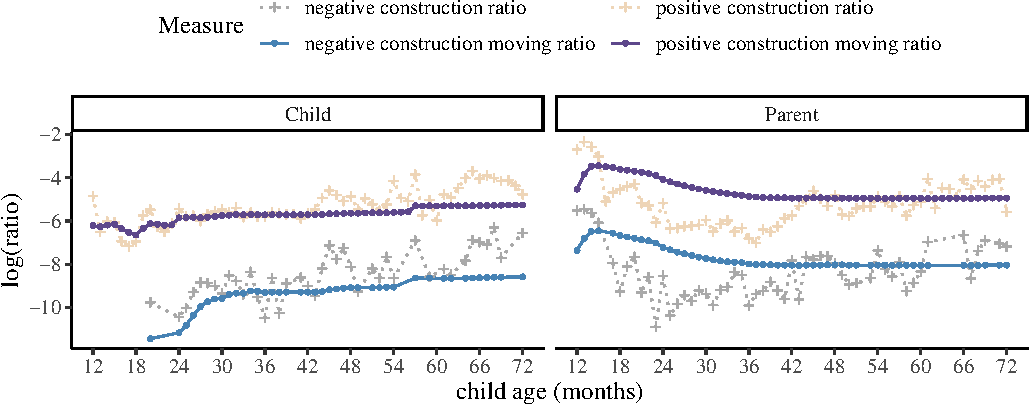
\includegraphics{neg_construction_article_files/figure-latex/prohibition-1} 

}

\caption{Ratios and cumulative ratios for the production of prohibition at the sentence level for children between 12 to 72 months of age, and their parents.}\label{fig:prohibition}
\end{figure}

\begin{figure}[H]

{\centering 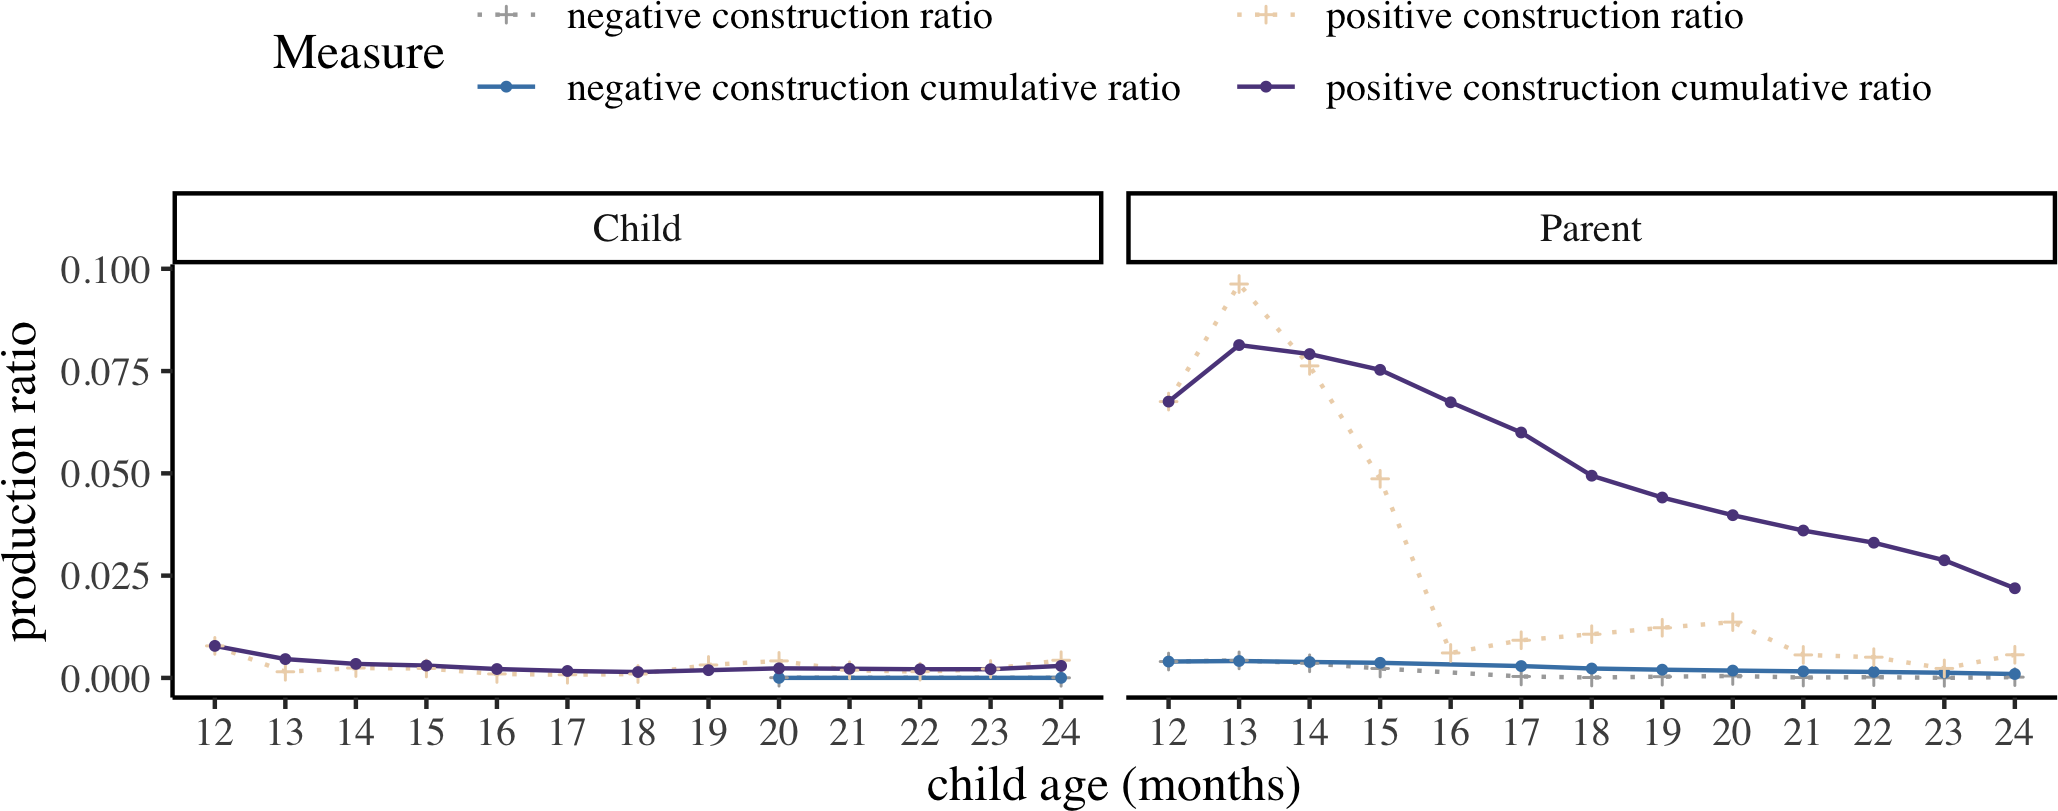
\includegraphics{neg_construction_article_files/figure-latex/prohibitionbegin-1} 

}

\caption{Ratios and cumulative ratios for the production of prohibition at the sentence level for children between 12 to 24 months of age, and their parents.}\label{fig:prohibitionbegin}
\end{figure}

At the discourse level, we selected \emph{No}-utterances with antecedents that were subjectless imperatives headed by a verb, excluding the following lemma forms: \emph{like}, \emph{want}, \emph{know}, \emph{think}, \emph{remember}, nor \emph{have}. This resulted in a total of 1,270 utterances (child: 8,968; parent: 17,643). As shown in Figure \ref{fig:prohibitiondiscourse}, children's usage of negation as a response particle to express prohibition is comparable to their productions at the sentence level. Their negative productions increases within the age range of 24 to 36 months, and parent production decreases when the children are between 12 to 36 months.

\begin{longtable}[]{@{}ll@{}}
\caption{\label{tab:disprohib} Example antecedents imperatives and discourse level negation in parents' and children's productions}\tabularnewline
\toprule
Antecedent & Utterance \\
\midrule
\endfirsthead
\toprule
Antecedent & Utterance \\
\midrule
\endhead
Parent: \emph{put away your toys} & Child: \emph{no mommy I like these} \\
\bottomrule
\end{longtable}

\begin{figure}[H]

{\centering 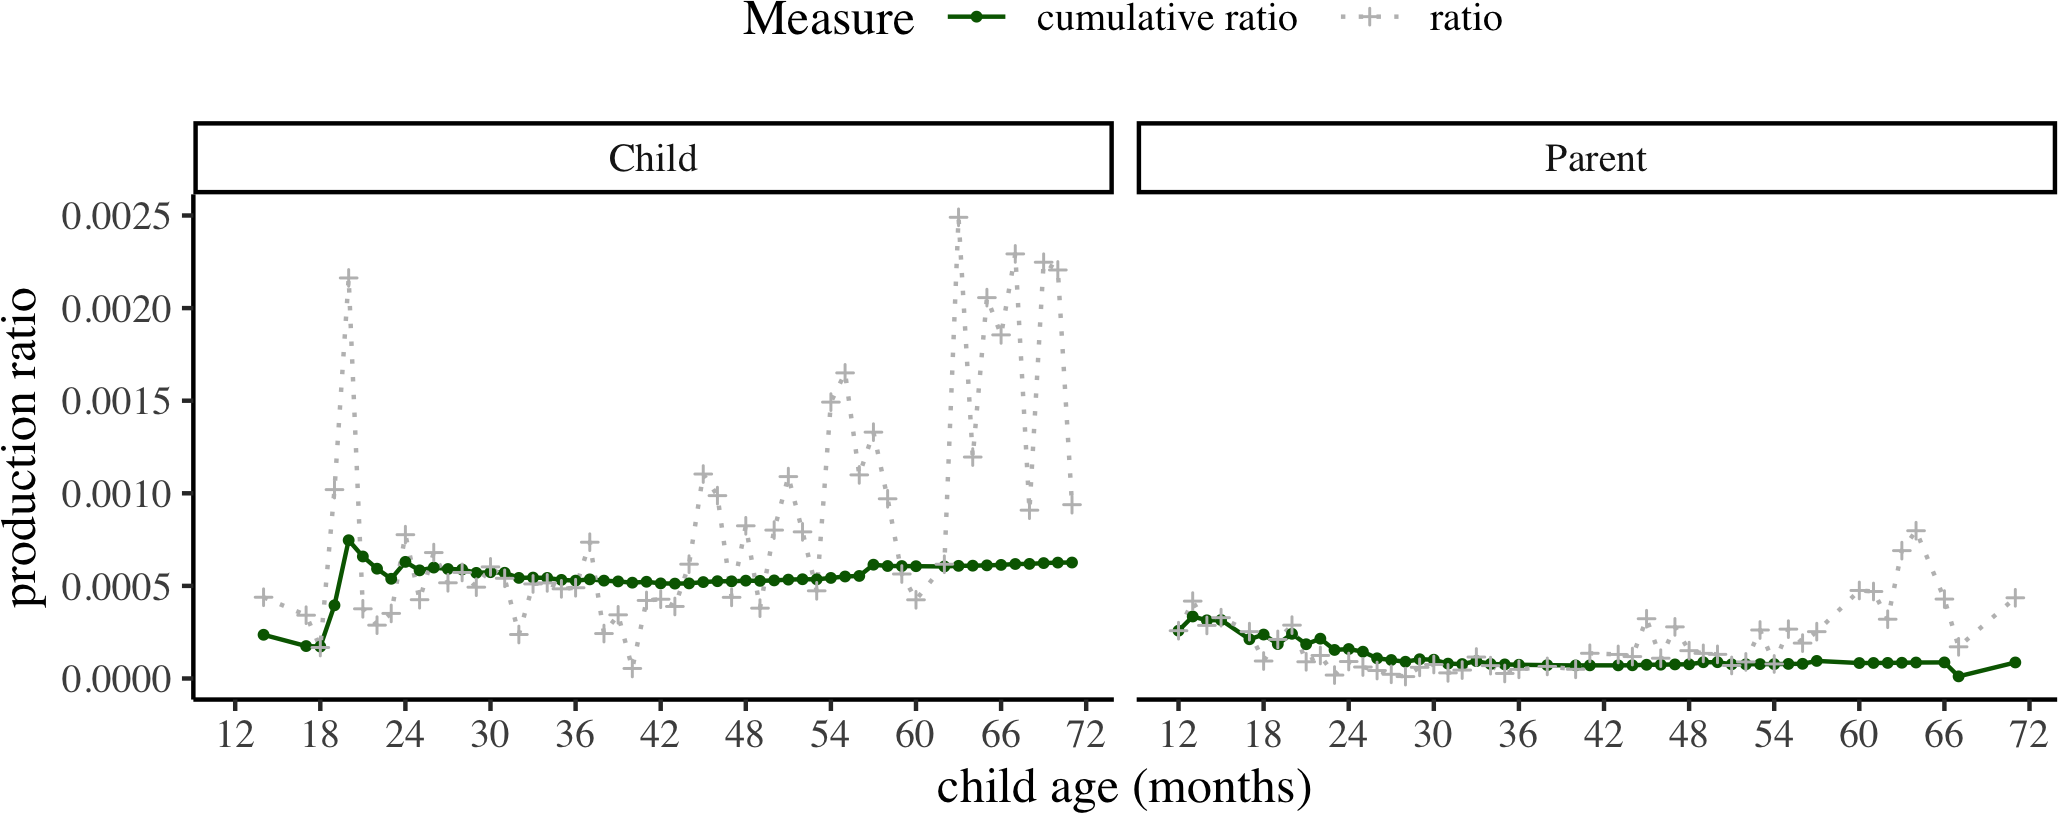
\includegraphics{neg_construction_article_files/figure-latex/prohibitiondiscourse-1} 

}

\caption{Ratios and cumulative ratios for the production of prohibition at the discourse level for children between 12 to 72 months of age, and their parents.}\label{fig:prohibitiondiscourse}
\end{figure}

\begin{figure}[H]

{\centering 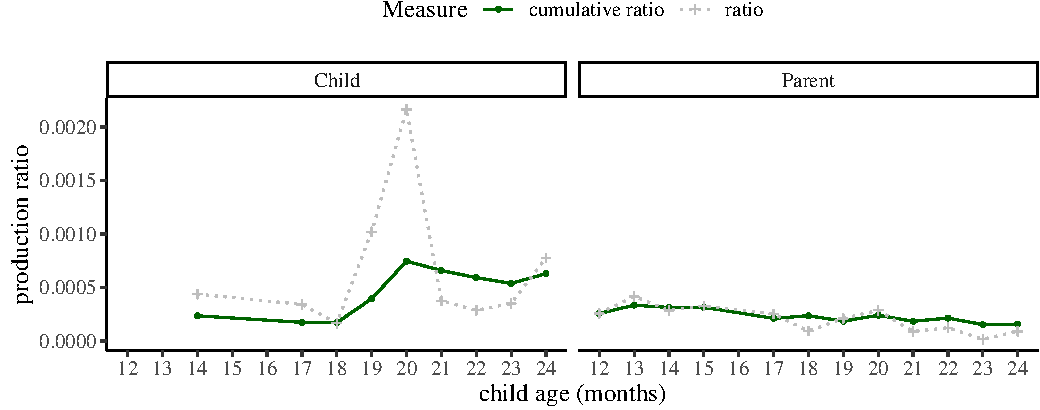
\includegraphics{neg_construction_article_files/figure-latex/prohibitiondiscoursebegin-1} 

}

\caption{Ratios and cumulative ratios for the production of prohibition at the discourse level for children between 12 to 24 months of age, and their parents.}\label{fig:prohibitiondiscoursebegin}
\end{figure}

\hypertarget{inability}{%
\subsubsection{Inability}\label{inability}}

For the function of inability, we analyzed instances with head verbs that are modified by the modal auxiliaries \emph{can} and \emph{could}. If the head verb was also modified by a negative morpheme, we classified it as negative. Otherwise, we considered it positive. Cases without a subject (e.g.~``can't play'') or with subjects that were not first person singular (e.g.~``you can't do that,'' ``this can't go in the box'') were excluded. This is because such cases often yield readings other than ``(in)ability.'' Depending on the larger context, they could be deontic (e.g.~``you are not allowed to do that'') or epistemic (e.g.~``it is not possible for it to go in the box''). To avoid this ambiguity and focus more on constructions that convey an individual's ability, we restricted our analyses only to cases with the first person singular subject \emph{I}. This led to 7,115 negative utterances (child: 3,917; parent: 3,198), and 14,433 positive utterances (child: 7,589; parent: 6,844). Table \ref{tab:inab} shows a few example of the cases we considered.

\begin{longtable}[]{@{}ll@{}}
\caption{\label{tab:inab} Examples of sentence-level inability (negative) and positive counterparts in children's speech.}\tabularnewline
\toprule
Inability (Negative) & Ability (Positive) \\
\midrule
\endfirsthead
\toprule
Inability (Negative) & Ability (Positive) \\
\midrule
\endhead
\emph{I can't see} & \emph{you could do it} \\
\emph{She can't go} & \emph{mommy could help me} \\
\bottomrule
\end{longtable}

Figure \ref{fig:inability} shows ratios and cumulative ratios of parents and children's productions of inability constructions as defined above. Similar to previous constructions, positive instances are generally more frequent than negative ones. Children produce inability negation more and more frequently between 18-36 months. After 36 months, their productions are stable and close to parent ratios.

\begin{figure}[H]

{\centering 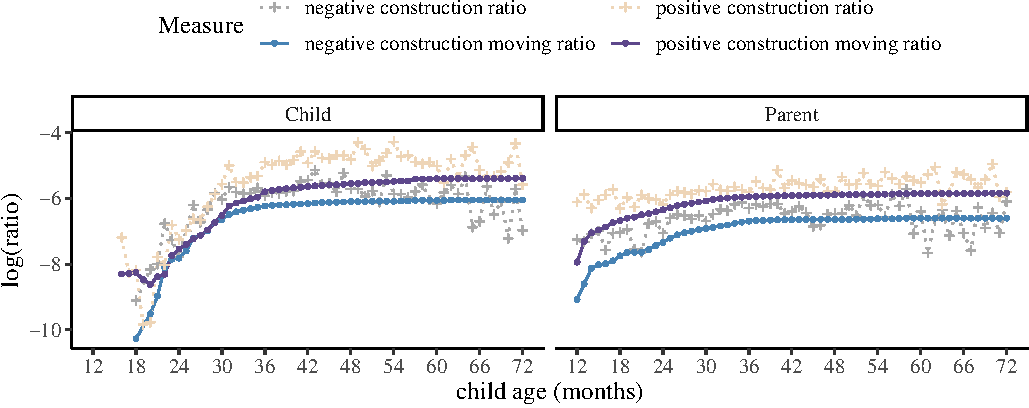
\includegraphics{neg_construction_article_files/figure-latex/inability-1} 

}

\caption{Ratios and cumulative ratios for the production of inability at the sentence level for children between 12 to 72 months of age, and their parents.}\label{fig:inability}
\end{figure}

\begin{figure}[H]

{\centering 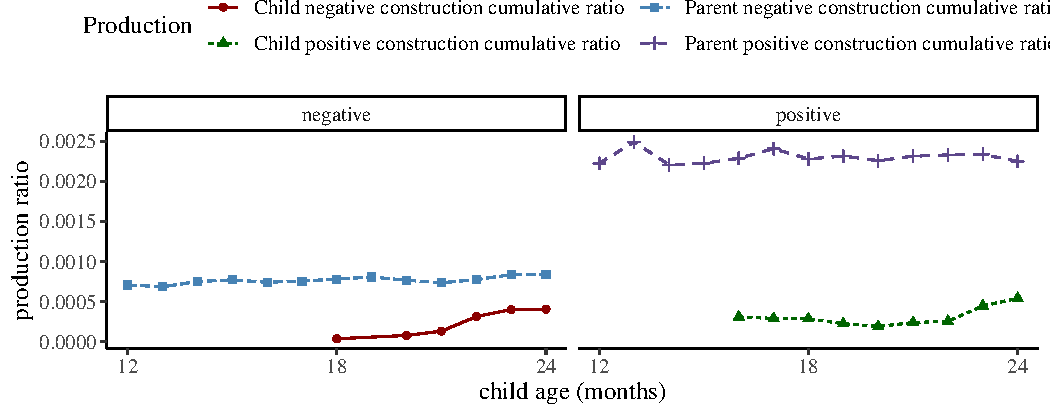
\includegraphics{neg_construction_article_files/figure-latex/inabilitybegin-1} 

}

\caption{Ratios and cumulative ratios for the production of inability at the sentence level for children between 12 to 24 months of age, and their parents.}\label{fig:inabilitybegin}
\end{figure}

At the discourse level, we selected utterances with the negative particle \emph{no} in response to antecedents that had a similar structure to the inability construction defined above. This yielded a total of 1,275 negative utterances (child: 11,506; parent: 10,042). Figure \ref{fig:inabilitydiscourse} shows the ratios and the cumulative ratios for parents' and children's production of discourse level inability construction. Considering cumulative ratios, children's productions gradually increase from 24 to 36 months and stabalizes after 36 months at a similar rate to that of parent's.

\begin{figure}[H]

{\centering 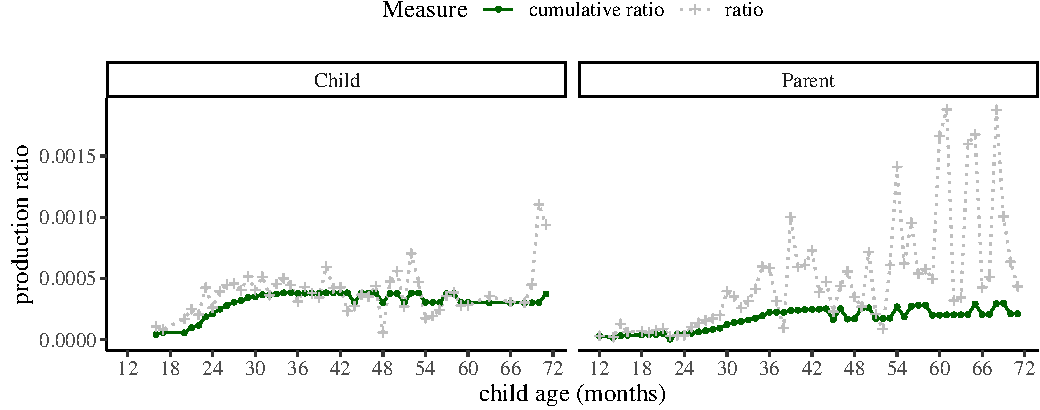
\includegraphics{neg_construction_article_files/figure-latex/inabilitydiscourse-1} 

}

\caption{Ratios and cumulative ratios for the production of inability at the discourse level for children between 12 to 72 months of age, and their parents.}\label{fig:inabilitydiscourse}
\end{figure}

\begin{figure}[H]

{\centering 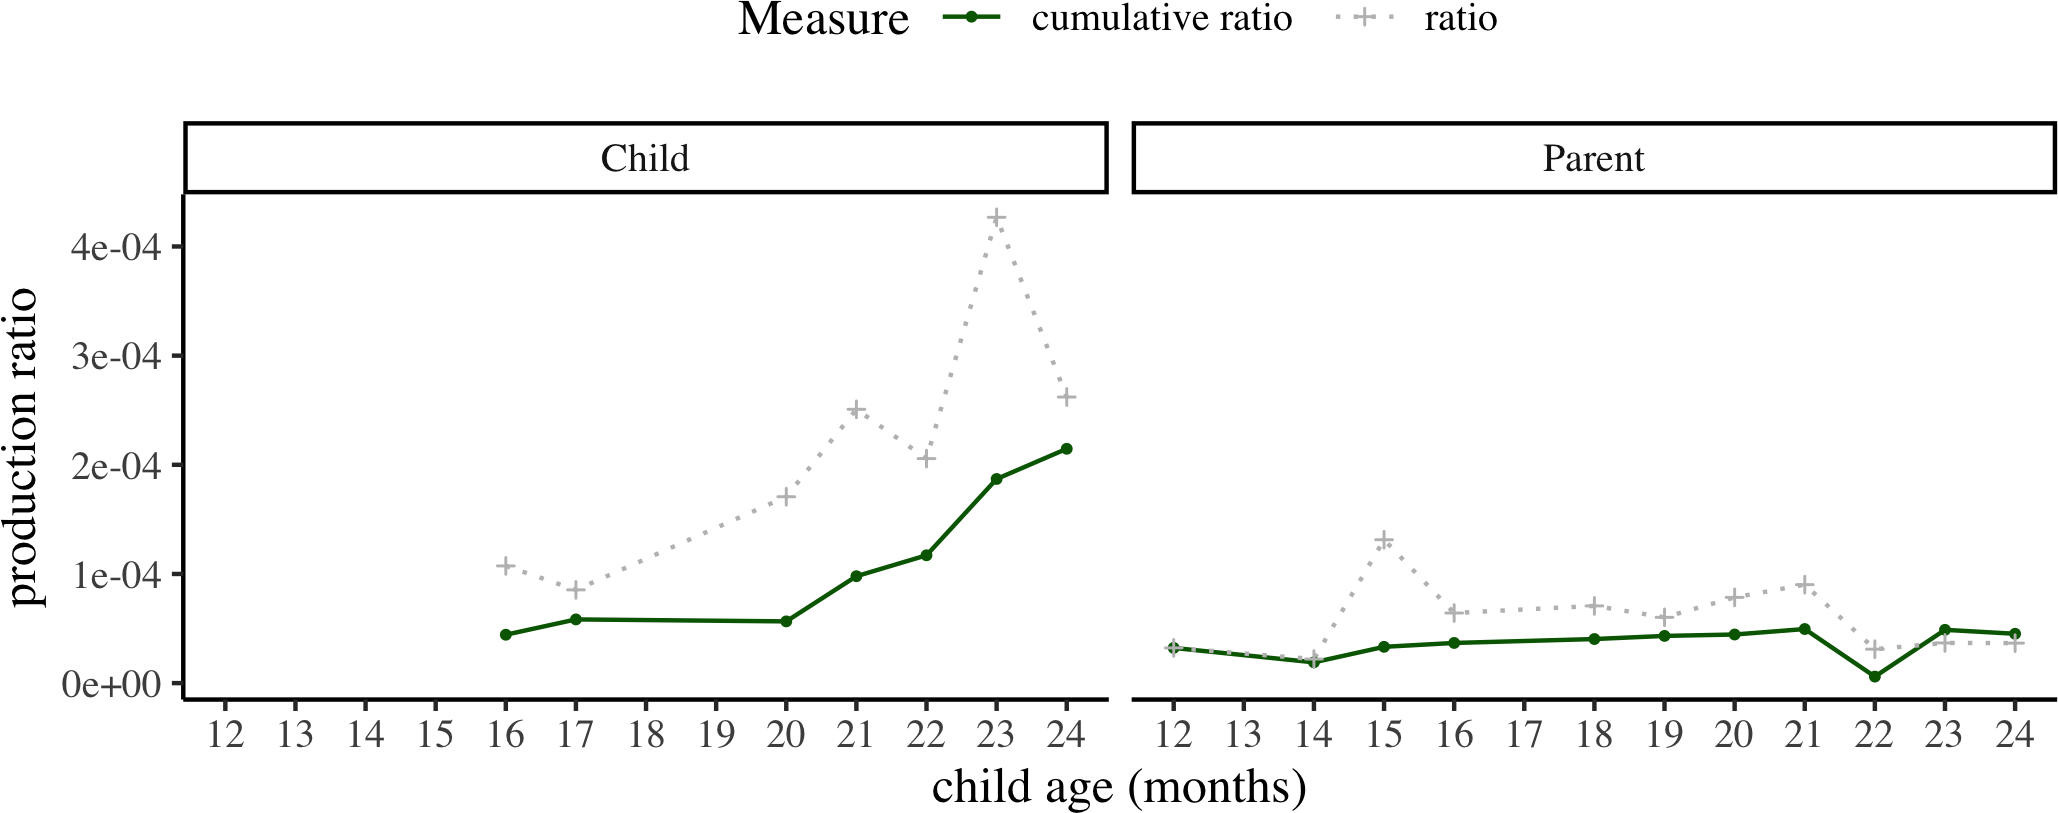
\includegraphics{neg_construction_article_files/figure-latex/inabilitydiscoursebegin-1} 

}

\caption{Ratios and cumulative ratios for the production of inability at the discourse level for children between 12 to 24 months of age, and their parents.}\label{fig:inabilitydiscoursebegin}
\end{figure}

\hypertarget{labeling}{%
\subsubsection{Labeling}\label{labeling}}

To capture the function of labeling at the sentence level, we concentrated on copula structures in which the predicate is a nominal or an adjectival phrase. Specifically, the nominal predicates exclude possessive pronouns in order to not overlap with the communicative function of possession (see below). We considered instances where the predicate is modified by negative morphemes as negative, and others as positive. To also avoid overlap with cases of non-existence, none of the utterances contained expletives (e.g.~``there is no book''). This resulted in a total of 36,410 negative utterances (Child: 6,193; Parent: 30,217), and 484,679 positive utterances (Child: 121,107; Parent: 363,572).

\begin{longtable}[]{@{}ll@{}}
\caption{\label{tab:label} Examples of sentence-level labeling (negative) and positive counterparts in children's speech.}\tabularnewline
\toprule
Labeling (Negative) & Labeling (Positive) \\
\midrule
\endfirsthead
\toprule
Labeling (Negative) & Labeling (Positive) \\
\midrule
\endhead
\emph{that's not a farmer} & \emph{this is a book} \\
\emph{this is not the book} & \emph{this is nice} \\
\emph{I'm not a heavy baby Mum} & \emph{it's a nice bowl} \\
\emph{It's no good} & \emph{she's pretty} \\
\bottomrule
\end{longtable}

Figure \ref{fig:learning} shows ratios and cumulative ratios for parent's and children's production of the labeling construction at the sentence level. In both parents and children, the frequency of positive counterparts is consistently higher than that of negative labeling instances. Children's productions of negative labeling increased between 18-36 months, and remained stable and close to the parent ratios after 36 months.

\begin{figure}[H]

{\centering 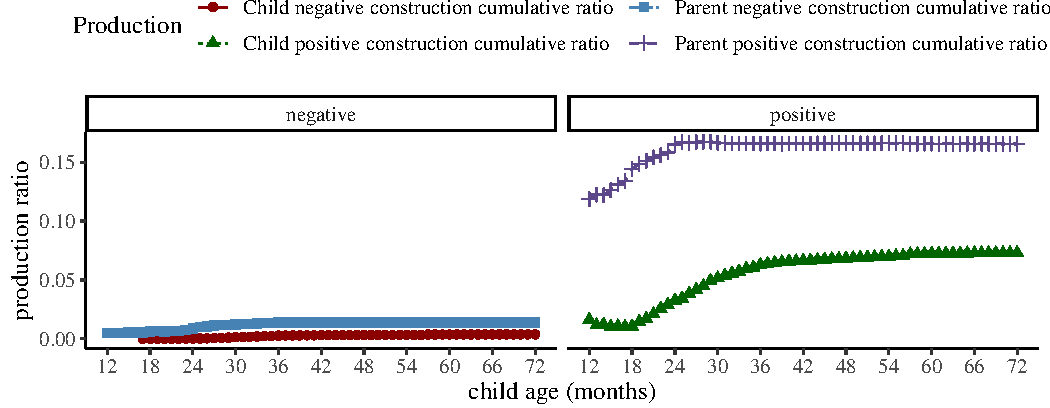
\includegraphics{neg_construction_article_files/figure-latex/learning-1} 

}

\caption{Ratios and cumulative ratios for the production of (negative) labeling at the sentence level for children between 12 to 72 months of age, and their parents.}\label{fig:learning}
\end{figure}

\begin{figure}[H]

{\centering 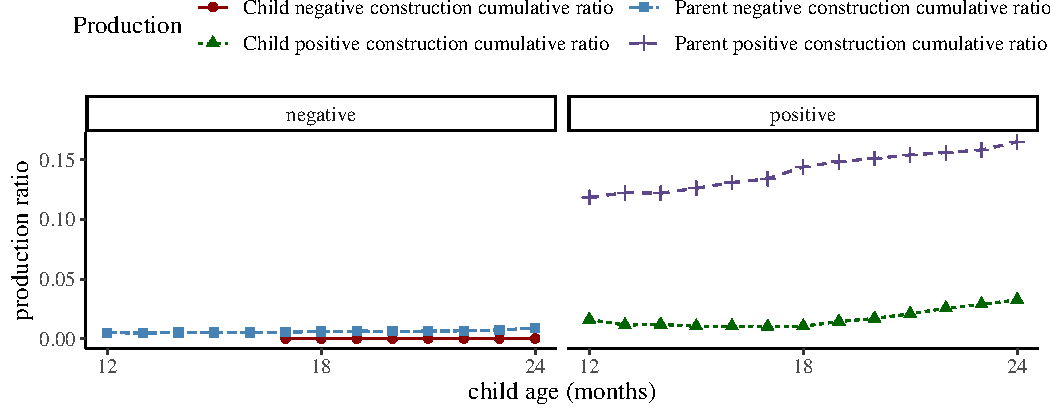
\includegraphics{neg_construction_article_files/figure-latex/learningbegin-1} 

}

\caption{Ratios and cumulative ratios for the production of (negative) labeling at the sentence level for children between 12 to 24 months of age, and their parents.}\label{fig:learningbegin}
\end{figure}

At the discourse level, we selected antecedent utterances with copula structures that combined with a nominal or an adjectival predicate. Table \ref{tab:dislabel} shows a few examples. We found 18,037 utterances (Child: 12,501; Parent: 5,536). Figure \ref{fig:learningdiscourse} shows the log ratios and cumulative ratios for labeling instances at the discourse level. Children used negation to respond to labeling utterances more frequently between 18 to 30 months. After 30 months, children's productions of negative labeling continues to increase but remains close to parents' level more generally.

\begin{longtable}[]{@{}ll@{}}
\caption{\label{tab:dislabel} Examples of discourse-level labeling (negative) and their antecedents in parents' and children's speech.}\tabularnewline
\toprule
Antecedent & Utterance \\
\midrule
\endfirsthead
\toprule
Antecedent & Utterance \\
\midrule
\endhead
Parent: \emph{is this one good} & Child: \emph{no it's not} \\
Parent: \emph{are you a captain} & Child: \emph{no I'm not} \\
Child: \emph{that's the one} & Parent: \emph{no it's the green one} \\
Child: \emph{this is the key} & Parent: \emph{no no} \\
\bottomrule
\end{longtable}

\begin{figure}[H]

{\centering 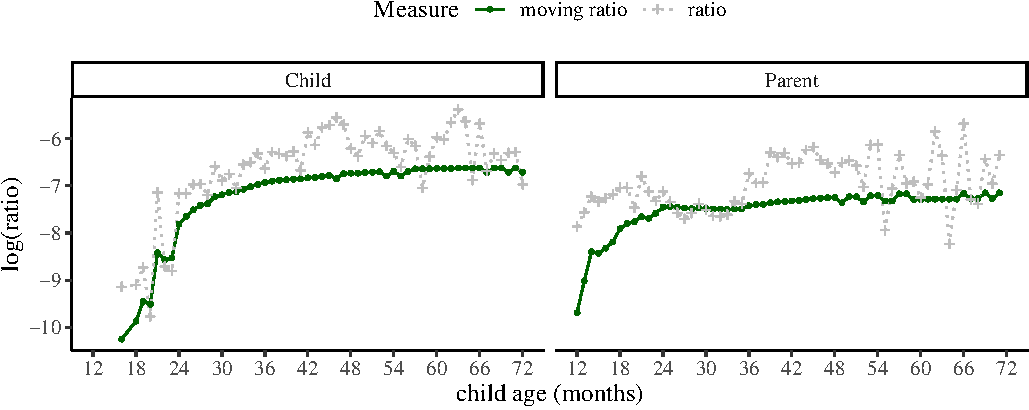
\includegraphics{neg_construction_article_files/figure-latex/learningdiscourse-1} 

}

\caption{Ratios and cumulative ratios for the production of (negative) labeling at the discourse level for children between 12 to 72 months of age, and their parents.}\label{fig:learningdiscourse}
\end{figure}

\begin{figure}[H]

{\centering 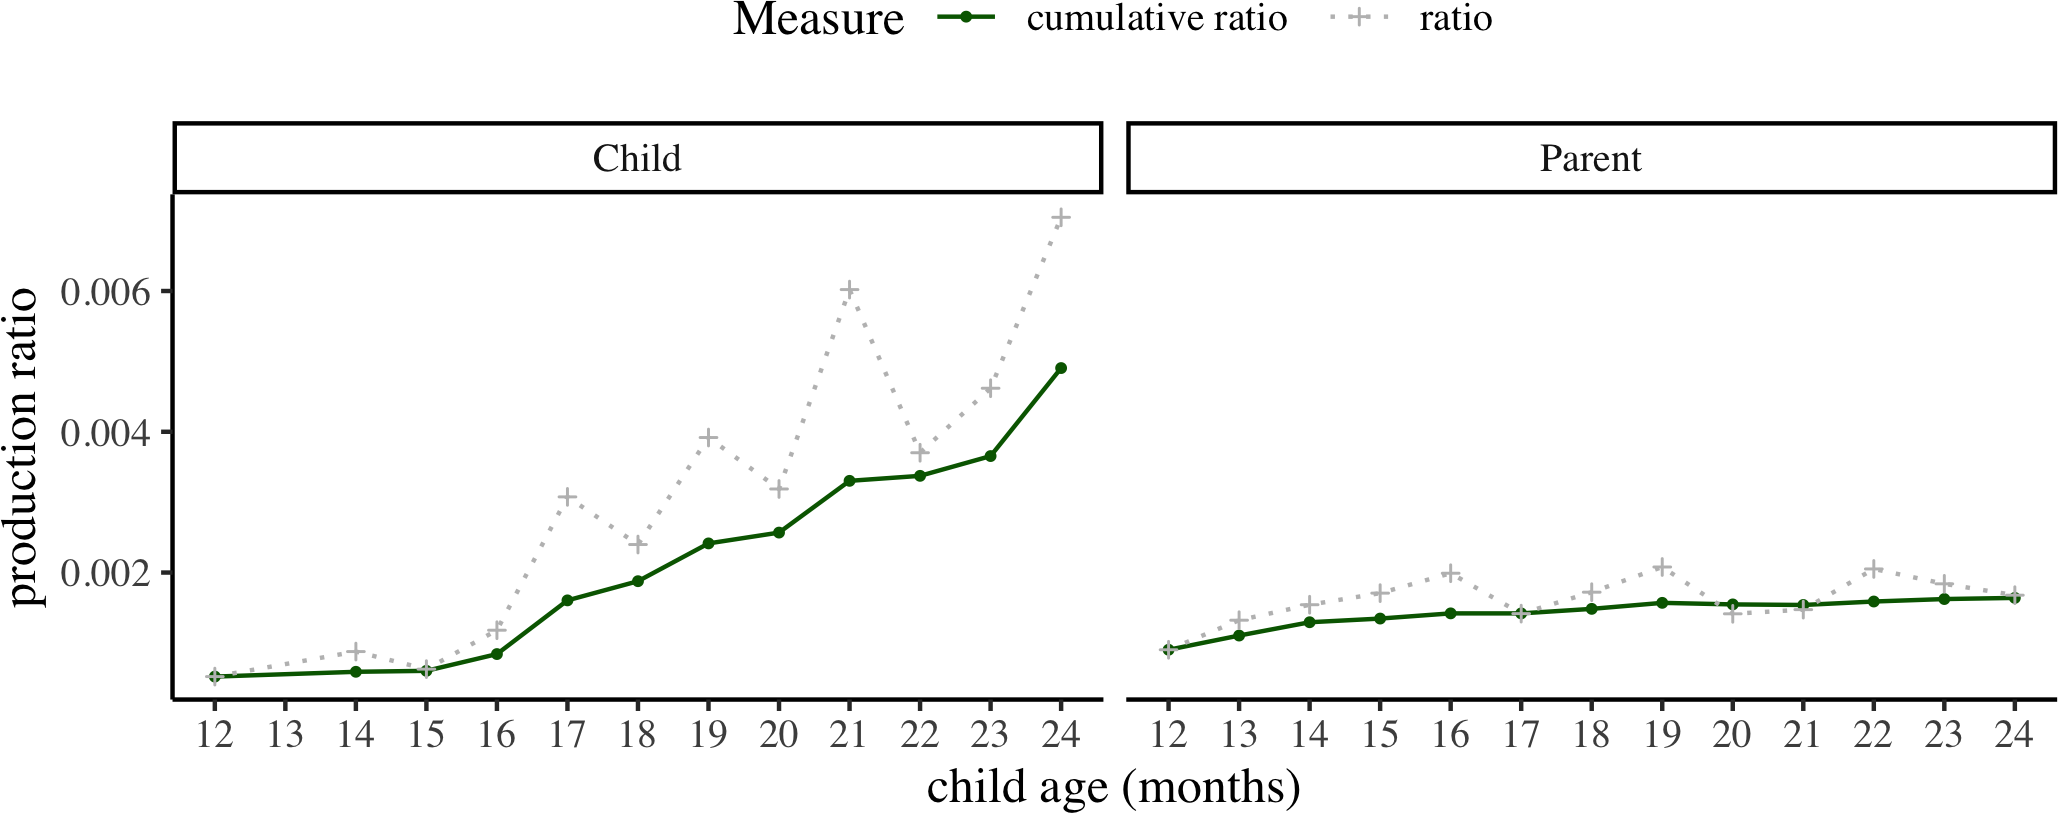
\includegraphics{neg_construction_article_files/figure-latex/learningdiscoursebegin-1} 

}

\caption{Ratios and cumulative ratios for the production of (negative) labeling at the discourse level for children between 12 to 24 months of age, and their parents.}\label{fig:learningdiscoursebegin}
\end{figure}

\hypertarget{epistemic-negation}{%
\subsubsection{Epistemic Negation}\label{epistemic-negation}}

Previous studies have reported instances in which children combined negative morphemes with mental state verbs such as \emph{know}, \emph{think}, and \emph{remember} to express ``epistemic negation'' (Choi, 1988). For defining epistemic constructions we also focused on these three verbs. For sentence level epistemic negation, we analyzed negative utterances where these verbs were modified by negative morphemes, possibly after combining with an auxiliary verb like \emph{do}. Table \ref{tab:epistem} shows a few examples. Instances where the speaker asked about or describes the negative epistemic state of another speaker were also included, leading to 31,696 negative utterances in total (child: 9,852; parent: 21,844). For the positive counterparts, we selected instances with the same head verbs except that these verbs were not modified by negation. This resulted in a total of 95,679 negative utterances (child: 16,322; parent: 79,357).

\begin{longtable}[]{@{}ll@{}}
\caption{\label{tab:epistem} Examples of sentence-level epistemic negation and positive counterparts in children's speech.}\tabularnewline
\toprule
Epistemic (Negative) & Epistemic (Positive) \\
\midrule
\endfirsthead
\toprule
Epistemic (Negative) & Epistemic (Positive) \\
\midrule
\endhead
\emph{I not know} & \emph{I knows} \\
\emph{I didn't remember} & \emph{she remembers} \\
\emph{I don't think so} & \emph{he thinks this one is good} \\
\emph{She doesn't know this} & \emph{She knows about this} \\
\bottomrule
\end{longtable}

Figure \ref{fig:epistemic} shows log ratios and cumulative ratios of the epistemic construction as defined above in parents' and children's speech at the sentence level. Overall, positive epistemic utterances were more frequent than negative epistemic utterances, with the possible exception of \emph{know} for children. The production of negative utterances headed by \emph{know} was comparatively the highest among children, and became more frequent at an earlier age (17-18 months) compared to that of \emph{remember} (\textasciitilde19 months) or \emph{think} (\textasciitilde20 months). Across the three head verbs, children's productions with \emph{know} and \emph{remember} gradually approaches that of parents' around 30 - 36 months, whereas cases with the head verb \emph{think} tend to be produced less frequently by children.

\begin{figure}[H]

{\centering 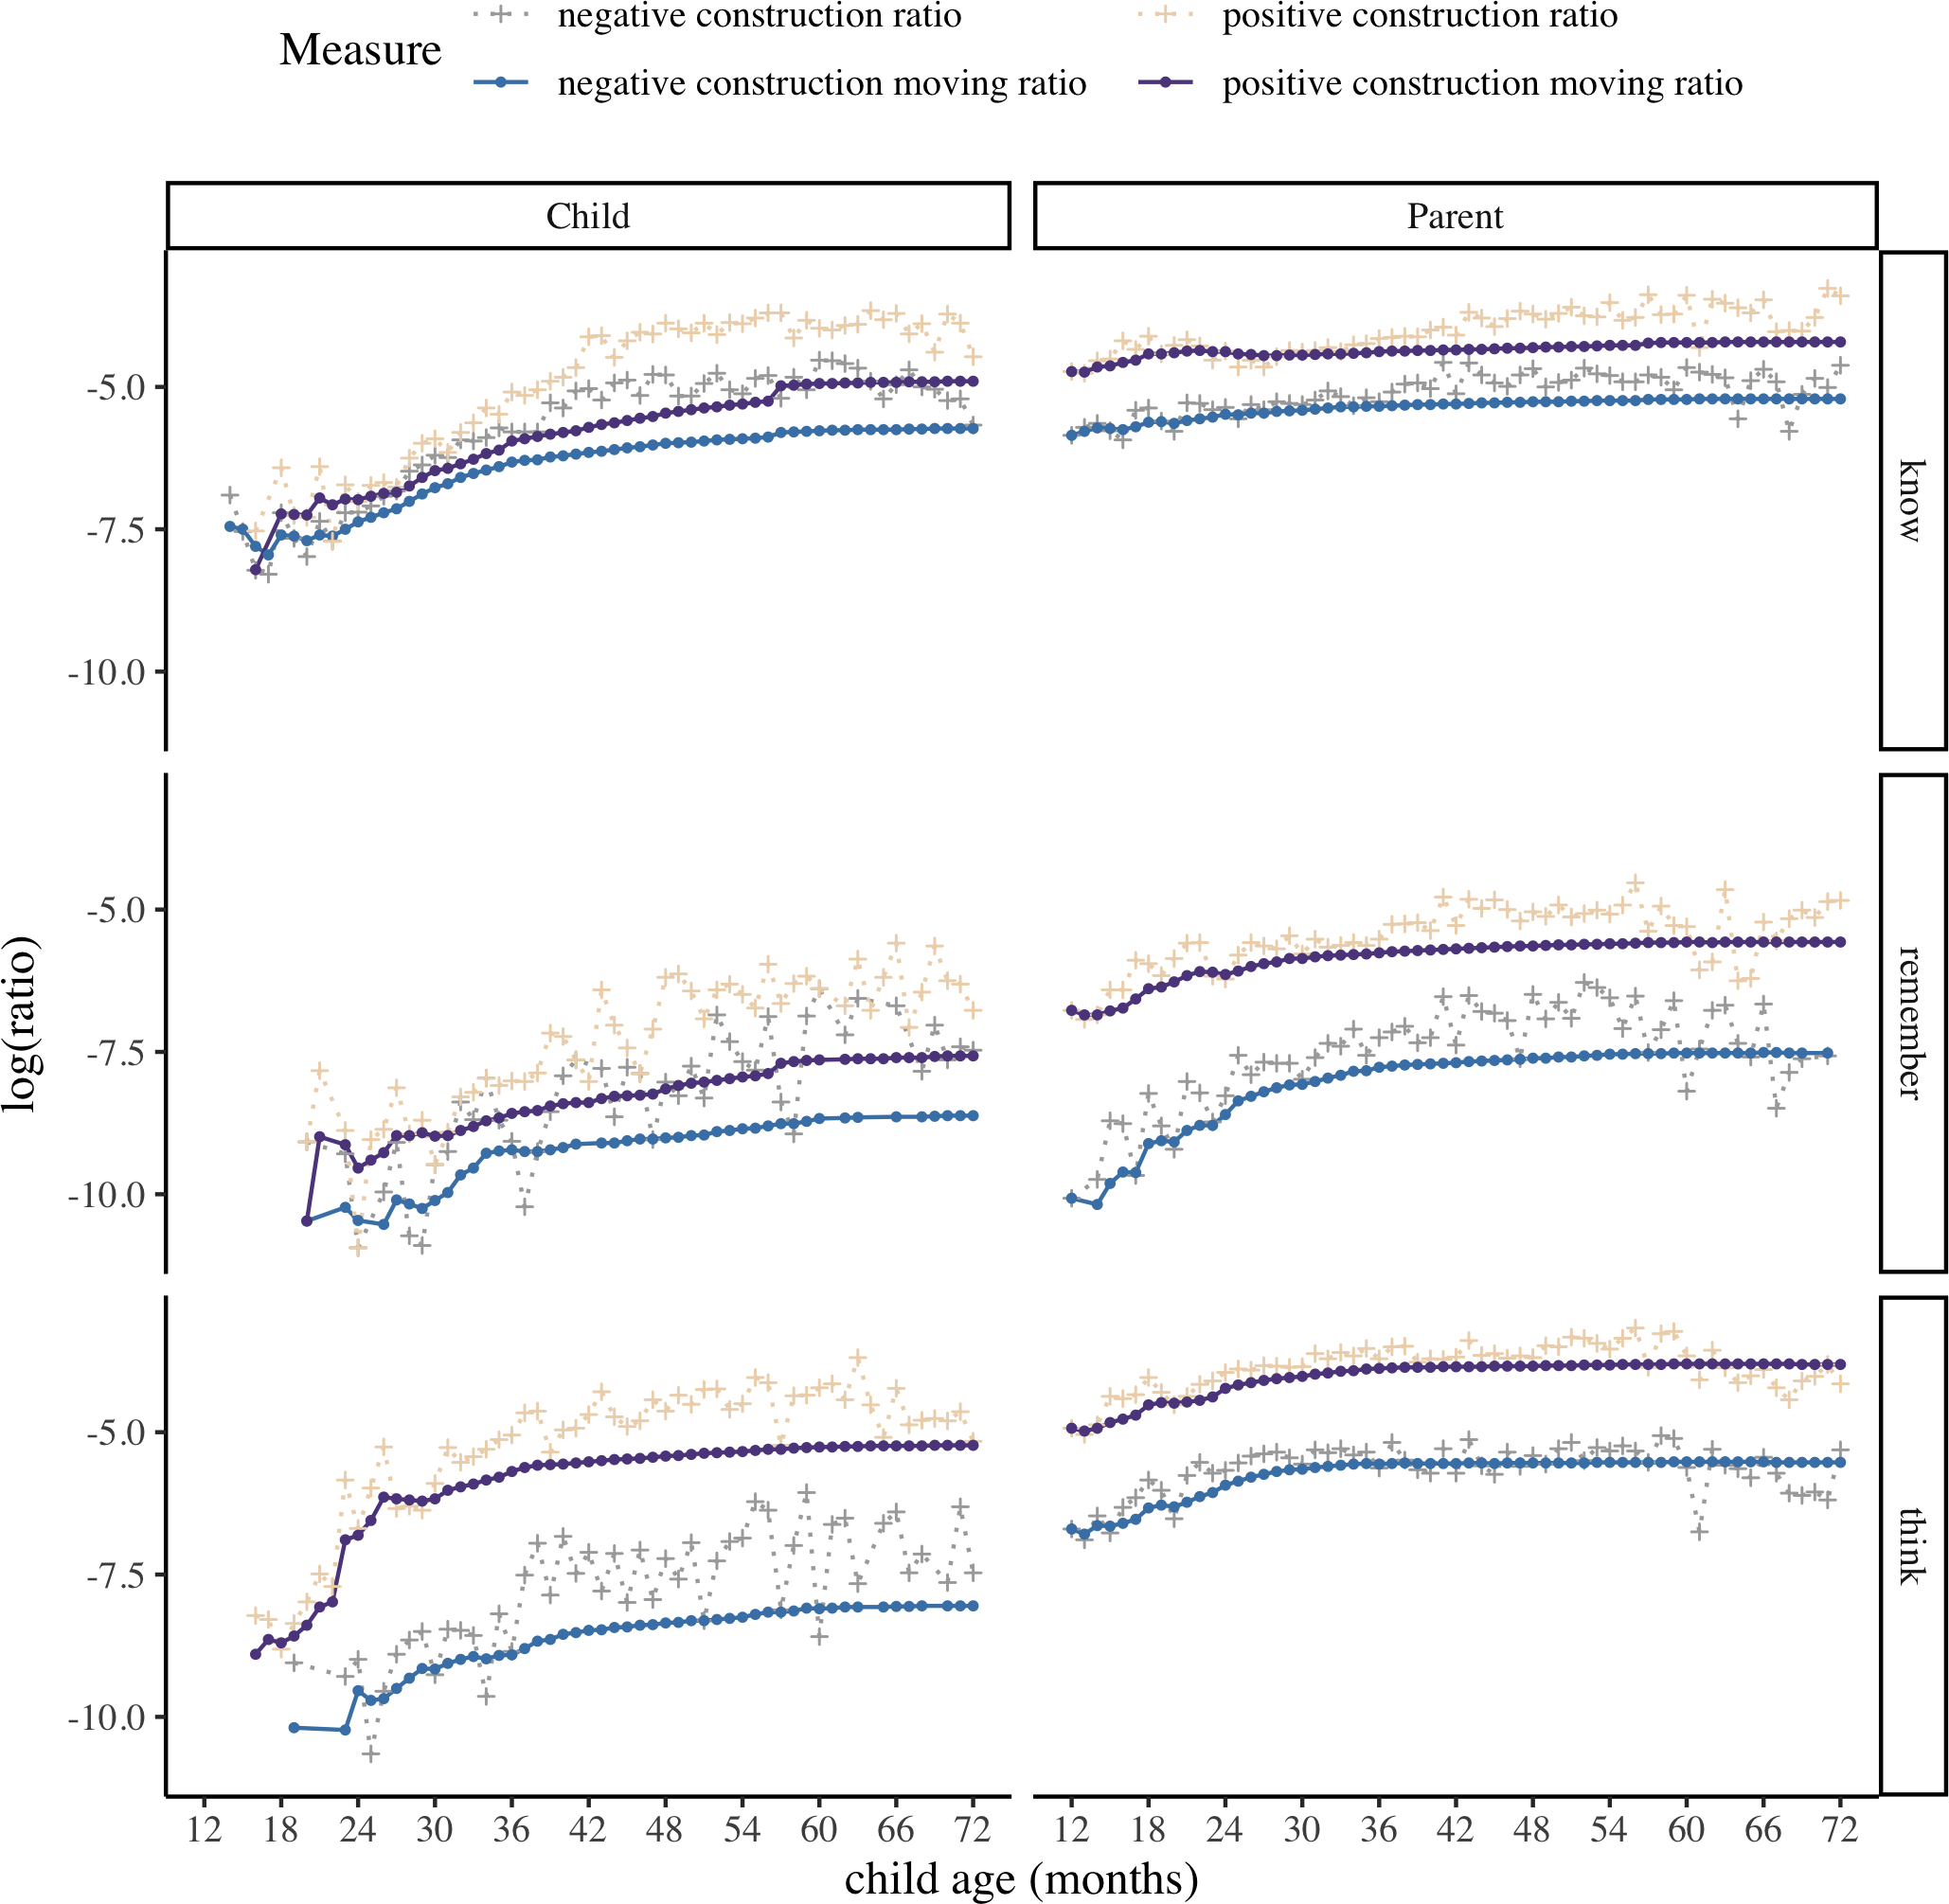
\includegraphics{neg_construction_article_files/figure-latex/epistemic-1} 

}

\caption{Ratios and cumulative ratios for the production of epistemic negation at the sentence level for children between 12 to 72 months of age, and their parents.}\label{fig:epistemic}
\end{figure}

\begin{figure}[H]

{\centering 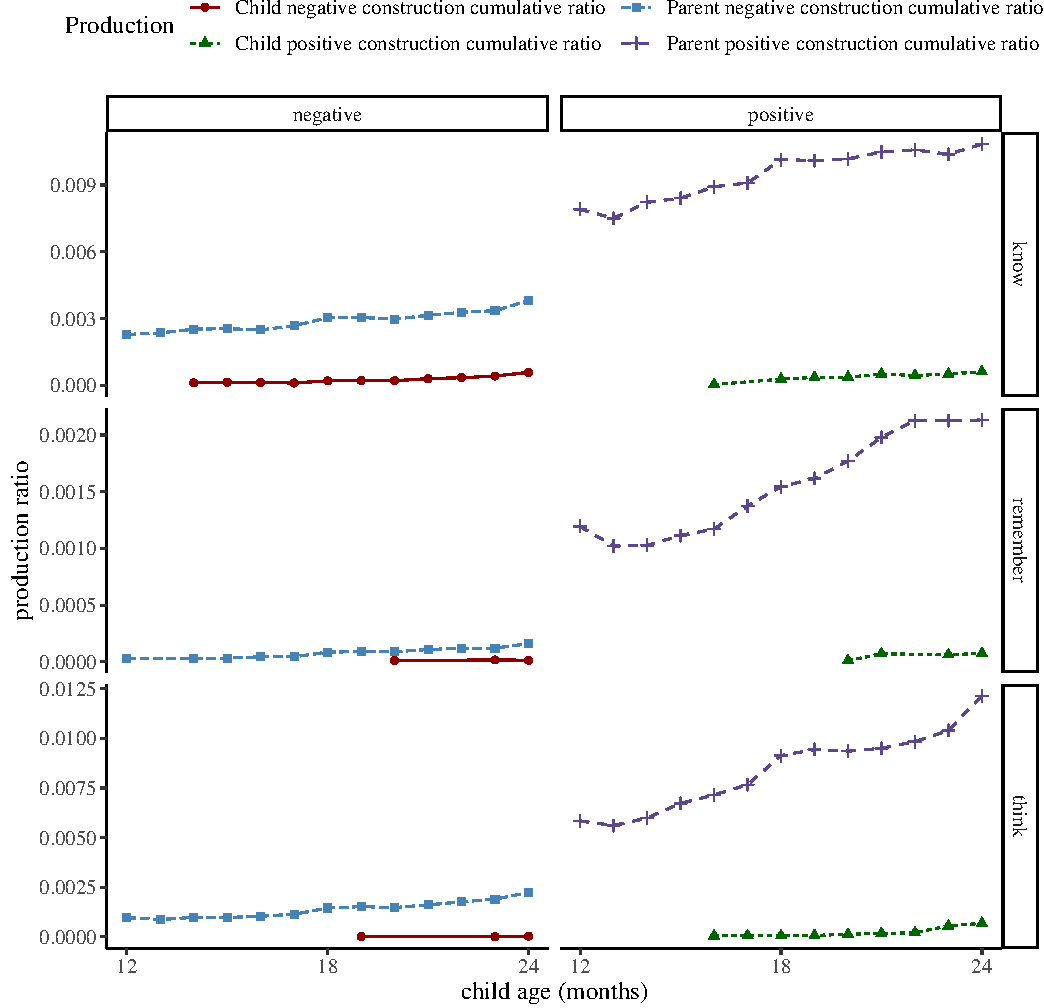
\includegraphics{neg_construction_article_files/figure-latex/epistemicbegin-1} 

}

\caption{Ratios and cumulative ratios for the production of epistemic negation at the sentence level for children between 12 to 24 months of age, and their parents.}\label{fig:epistemicbegin}
\end{figure}

For epistemic negation at the discourse level, we examined interactions in which the antecedent utterances took any of the three head verbs \emph{know}, \emph{remember} and \emph{think}, leading to a total of 5,695 utterances (child: 26,174; parent: 101,201). Figure \ref{fig:epistemicdiscourse} shows log ratios and cumulative ratios for epistemic negation at the discourse level. Children's productions increase rapidly between 24-36 months and after 36 months, they produce this construction close to parent levels.

\begin{longtable}[]{@{}ll@{}}
\caption{\label{tab:epistem} Examples of sentence-level epistemic negation and positive counterparts in children's speech.}\tabularnewline
\toprule
Epistemic (Negative) & Epistemic (Positive) \\
\midrule
\endfirsthead
\toprule
Epistemic (Negative) & Epistemic (Positive) \\
\midrule
\endhead
\emph{I not know} & \emph{I knows} \\
\emph{I didn't remember} & \emph{she remembers} \\
\emph{I don't think so} & \emph{he thinks this one is good} \\
\emph{She doesn't know this} & \emph{She knows about this} \\
\bottomrule
\end{longtable}

\begin{figure}[H]

{\centering 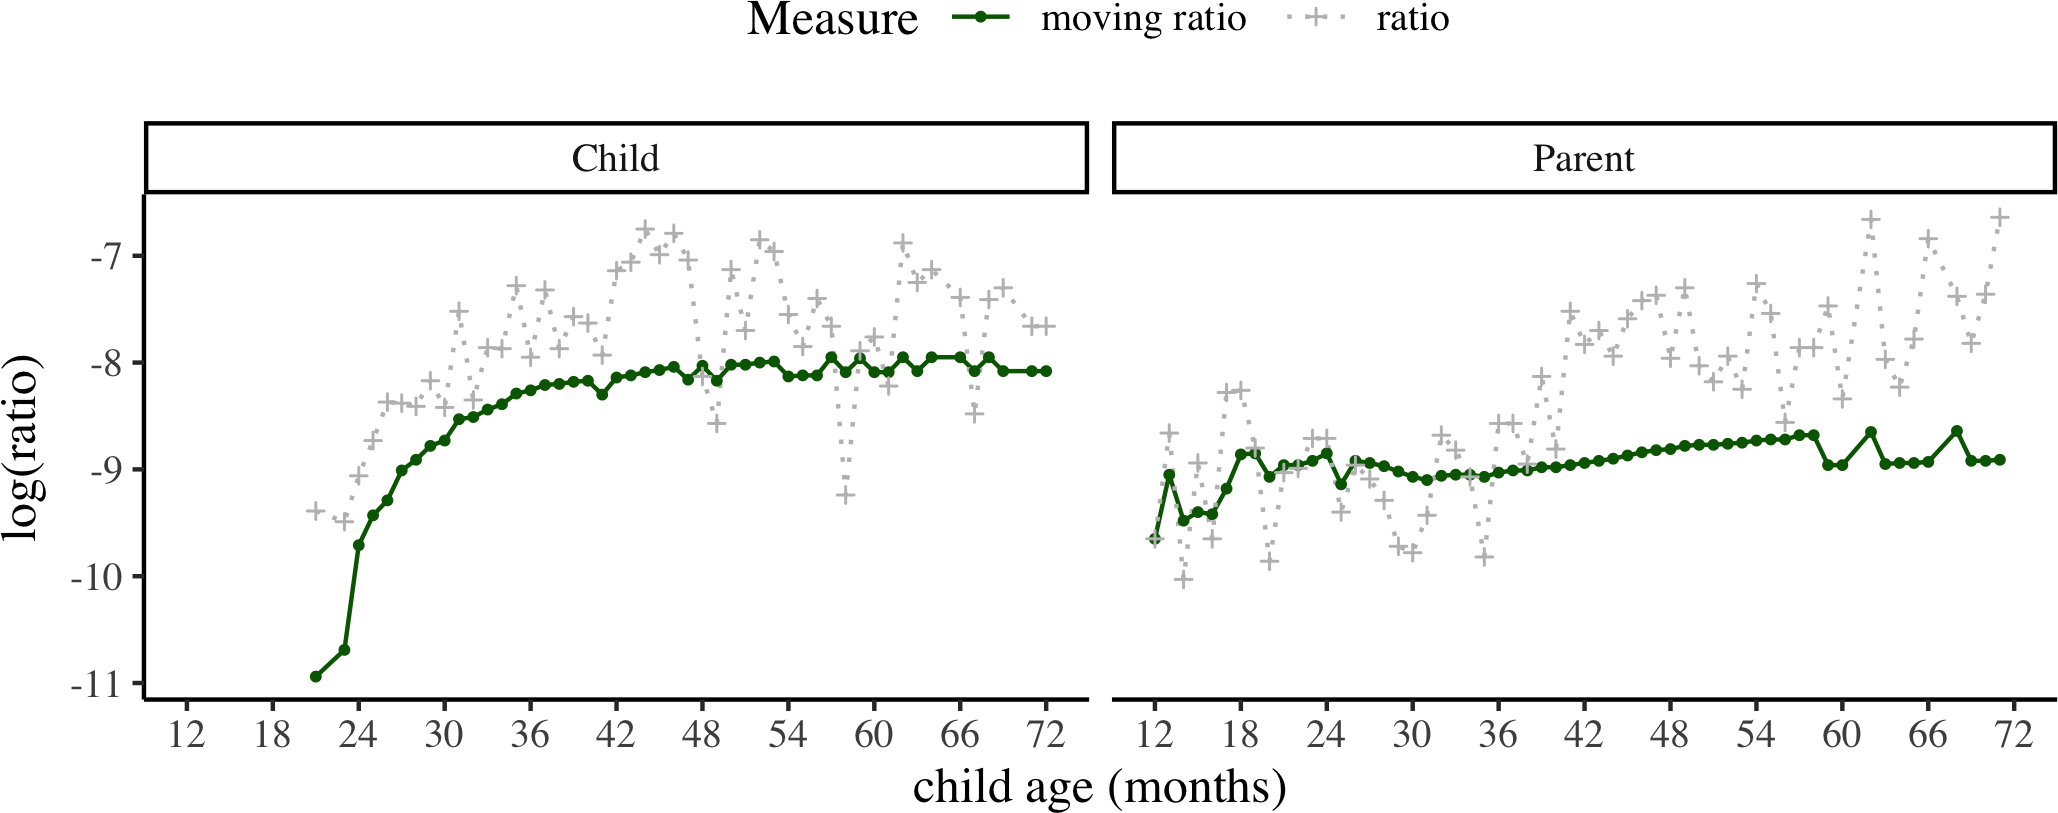
\includegraphics{neg_construction_article_files/figure-latex/epistemicdiscourse-1} 

}

\caption{Ratios and cumulative ratios for the production of epistemic negation at the discourse level for children between 12 to 72 months of age, and their parents.}\label{fig:epistemicdiscourse}
\end{figure}

\begin{figure}[H]

{\centering 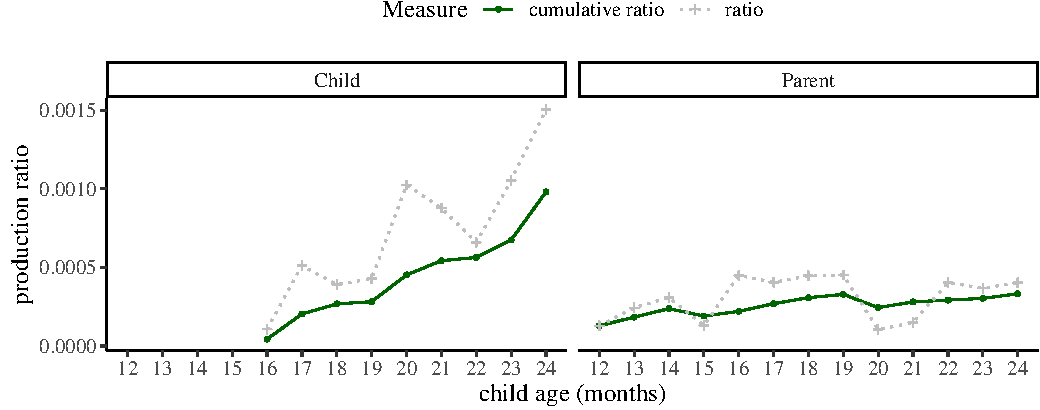
\includegraphics{neg_construction_article_files/figure-latex/epistemicdiscoursebegin-1} 

}

\caption{Ratios and cumulative ratios for the production of epistemic negation at the discourse level for children between 12 to 24 months of age, and their parents.}\label{fig:epistemicdiscoursebegin}
\end{figure}

\hypertarget{possession}{%
\subsubsection{Possession}\label{possession}}

The last function we explored was ``possession.'' At the syntactic level, for negative structures we selected cases where negative morphemes were combined with auxiliary verbs to modify a head verb with the lemma form \emph{have} and a POS tag of VERB. We also included individual noun phrases with possessive pronouns as heads and modified by negative morphemes. Table \ref{tab:possess} shows a few examples. Cases in which the syntactic head of the negative morphemes is a predicate of a copula verb (e.g.~``this is not mine'') were excluded to separate them from the function ``labeling.'' The number of negative utterances that were subjected to analysis for this function is 8,892 (child: 2,830; parent: 6,062). Again the positive counterparts share similar structures except with no negation, leading to a total of 86,665 (child: 27,730; parent: 58,935). One thing to note here is that for the positive structures with the head verb \emph{have}, we restricted to cases where the verb takes a direct object (with the dependency relation \emph{obj}). This is to avoid potential parsing errors of instances such as \emph{I have}, where the verb could ambiguously be an auxiliary.

\begin{longtable}[]{@{}ll@{}}
\caption{\label{tab:possess} Examples of sentence-level possession and positive counterparts in children's speech.}\tabularnewline
\toprule
Posession (Negative) & Posession (Positive) \\
\midrule
\endfirsthead
\toprule
Posession (Negative) & Posession (Positive) \\
\midrule
\endhead
\emph{I don't have it} & \emph{you have that} \\
\emph{you don't have my toy car} & \emph{she has it} \\
\emph{not mine} & \emph{hers} \\
\emph{not yours either} & \emph{mine mine mine} \\
\bottomrule
\end{longtable}

Figure \ref{fig:possession} shows log ratios and cumulative ratios of the negative and positive possession construction at the sentence level. The production trajectory for possession in child speech appears to have notable differences depending on what the negative morpheme modifies. With \emph{have} as the syntactic head, children increase their productions between 18-36 months, and stay close to parent levels of production after 36 months. However, for utterances headed by possessive pronouns, productions increase rapidly between 18-24 months and stays close to parent levels as early as 24 months of age.

\begin{figure}[H]

{\centering 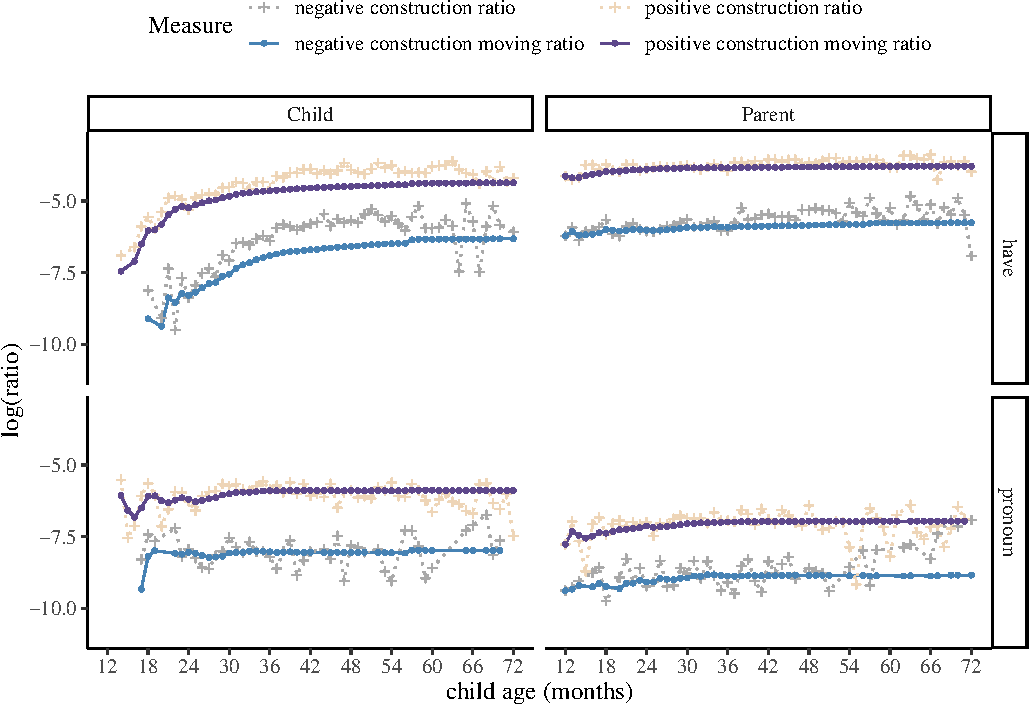
\includegraphics{neg_construction_article_files/figure-latex/possession-1} 

}

\caption{Ratios and cumulative ratios for the production of possession at the sentence level for children between 12 to 72 months of age, and their parents.}\label{fig:possession}
\end{figure}

\begin{figure}[H]

{\centering 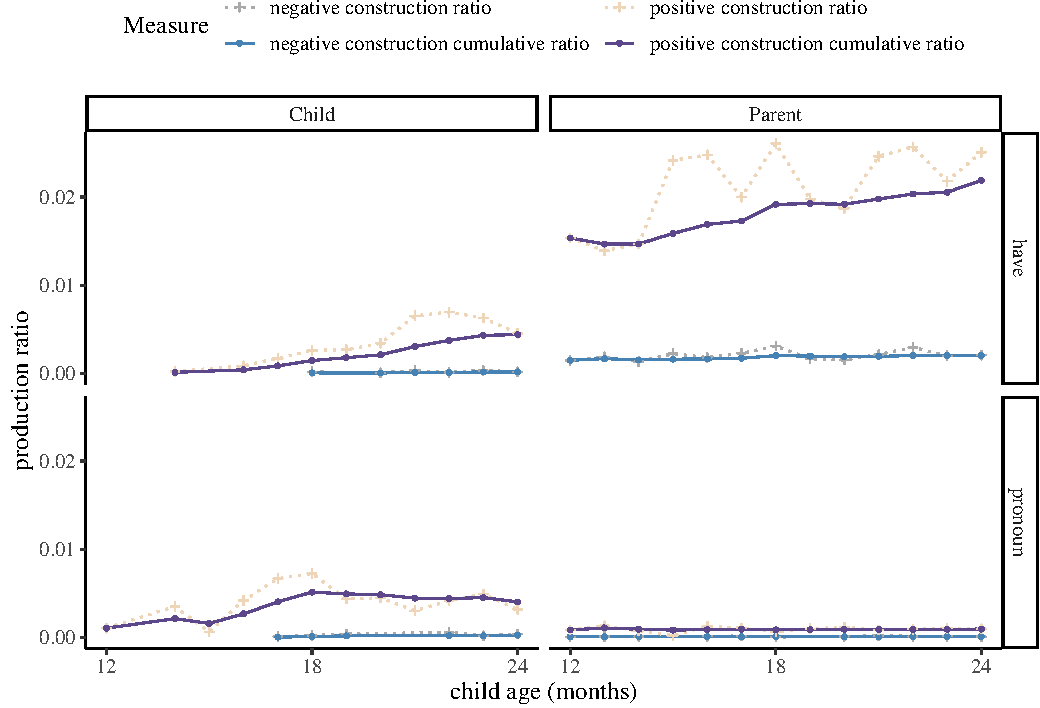
\includegraphics{neg_construction_article_files/figure-latex/possessionbegin-1} 

}

\caption{Ratios and cumulative ratios for the production of possession at the sentence level for children between 12 to 24 months of age, and their parents.}\label{fig:possessionbegin}
\end{figure}

At the discourse level, we selected antecedents to discourse level negative utterances (e.g.~\emph{no!}) which themselves had structures similar to both the negative and positive constructions at the syntactic level. Table \ref{tab:dispossess} provides a few examples and Figure \ref{fig:possessiondiscourse} shows log ratios and cumulative ratios of such utterances in parents' and children's speech. Overall, the production pattern for discourse level possession suggests that children produce such utterances frequently and at parents' level after 30 or 36 months of age.

\begin{longtable}[]{@{}ll@{}}
\caption{\label{tab:dispossess} Examples of discourse-level possession and their antecedents in parents' and children's speech.}\tabularnewline
\toprule
Antecedent & Utterance \\
\midrule
\endfirsthead
\toprule
Antecedent & Utterance \\
\midrule
\endhead
Parent: \emph{not yours} & Child: \emph{no it's mine mine} \\
Parent: \emph{do you still have that picture} & Child: \emph{no} \\
Child: \emph{I don't have the book} & Parent: \emph{no no mommy please read it to me} \\
Child: \emph{mommy has it} & Parent: \emph{no mommy gave it back to your auntie} \\
\bottomrule
\end{longtable}

\begin{figure}[H]

{\centering 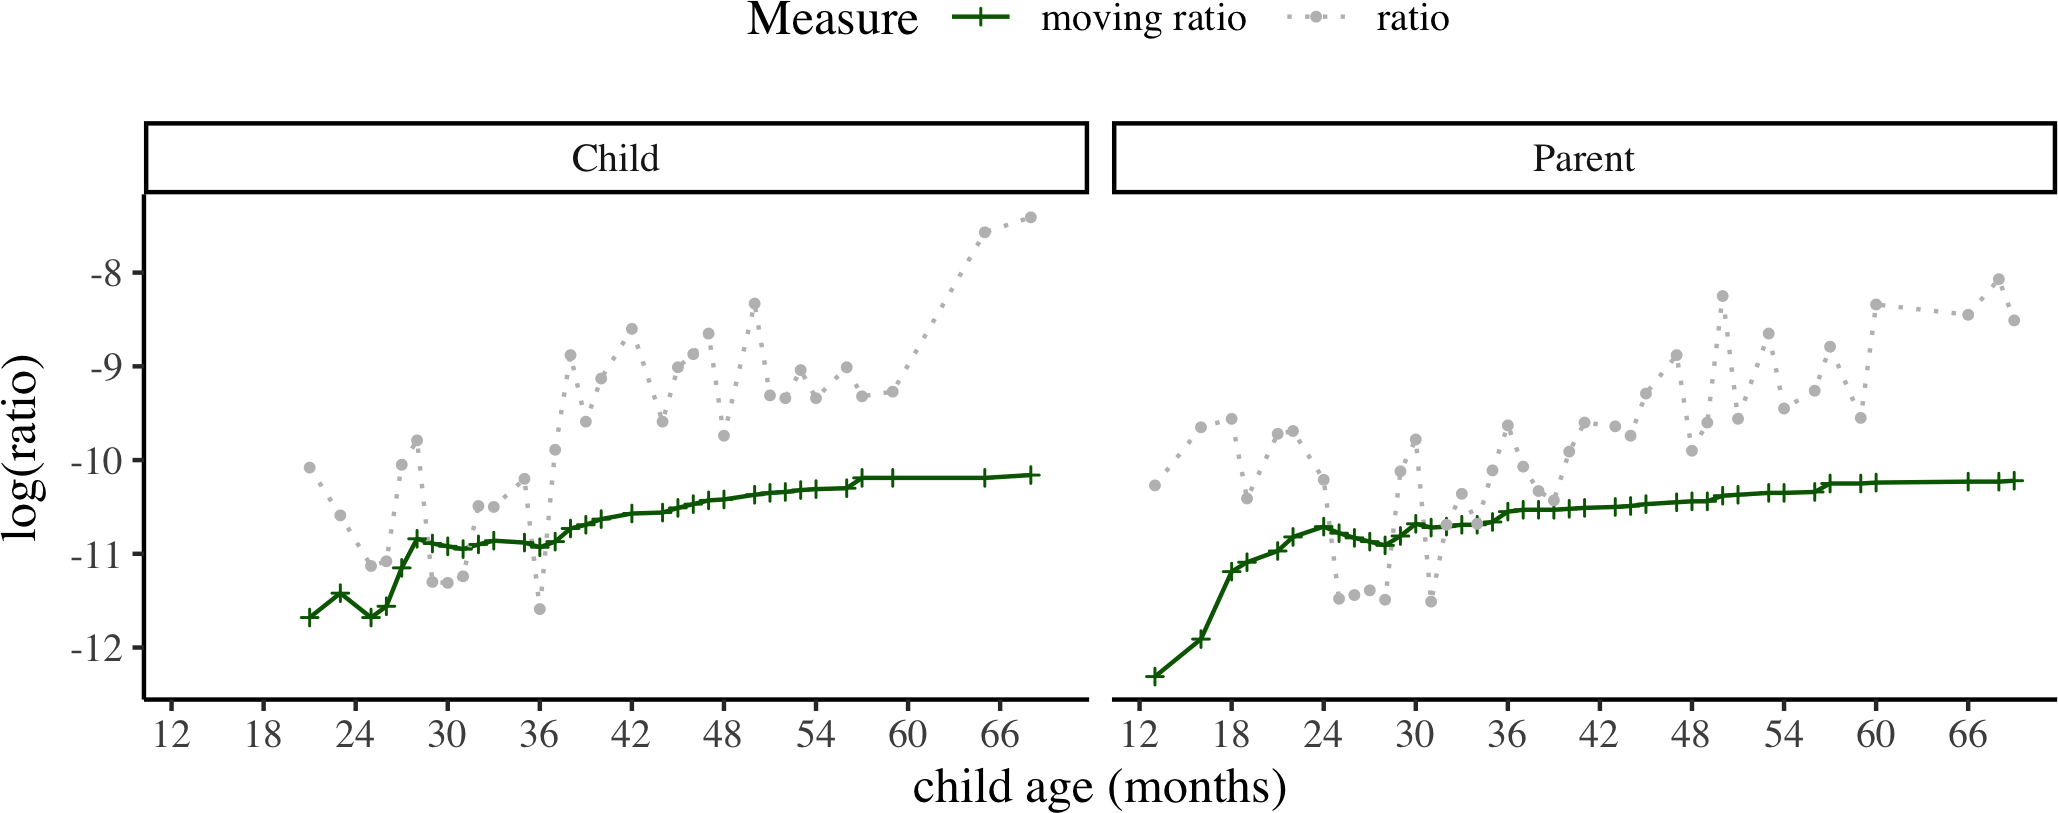
\includegraphics{neg_construction_article_files/figure-latex/possessiondiscourse-1} 

}

\caption{Ratios and cumulative ratios for the production of possession at the discourse level for children between 12 to 72 months of age, and their parents.}\label{fig:possessiondiscourse}
\end{figure}

\begin{figure}[H]

{\centering 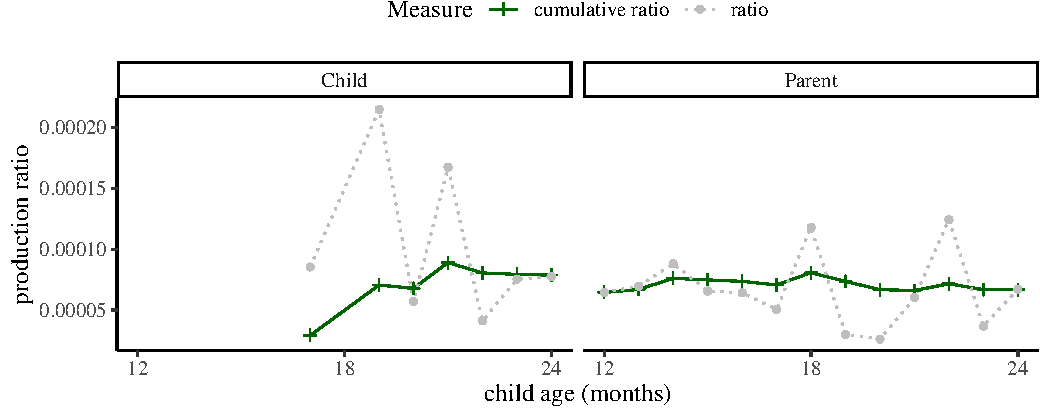
\includegraphics{neg_construction_article_files/figure-latex/possessiondiscoursebegin-1} 

}

\caption{Ratios and cumulative ratios for the production of possession at the discourse level for children between 12 to 24 months of age, and their parents.}\label{fig:possessiondiscoursebegin}
\end{figure}

\hypertarget{discussion}{%
\subsubsection{Discussion}\label{discussion}}

Figure \ref{fig:allneg} shows the log cumulative ratios of all our negative constructions at the sentence level. Looking at parents' productions (right panel), we see that for most constructions, parents produce them at constant rates across age bins. A notable exception to this trend is ``prohibition,'' which starts close to the most frequent constructions at 12-18 months of age and ends up as the least frequently used construction around 42-72 months. One obvious reason for this trend is that when children are younger, parents may need to guide children's actions through prohibitions a lot more frequently than later in the child's life. Looking at children's productions (left panel), we see that the production of most constructions begins in the 12-24 age range. Two constructions, non-existence and prohibition, seem to show some delay. With non-existence, even though there are examples between 18-24 months, there is a discontinuity around 24 months instead of a slow and steady increase seen in other functions. This may be partly due to the samples available at that age range and with more data a clearer pattern may emerge. With prohibitions, we see a relatively smooth pattern. Children start to produce them later than other functions (between 24-30 months) and its rate of production stays below parents' levels. This pattern may be because prohibitions develop later than other functions, or it may have socio-pragmatic explanations. It is possible that parent-child interaction does not provide many contexts for children to prohibit parents. Nevertheless by 36 months of age, most constructions are produced close to parents' levels. Again prohibitions seem to be exceptional.

\begin{figure}[H]

{\centering 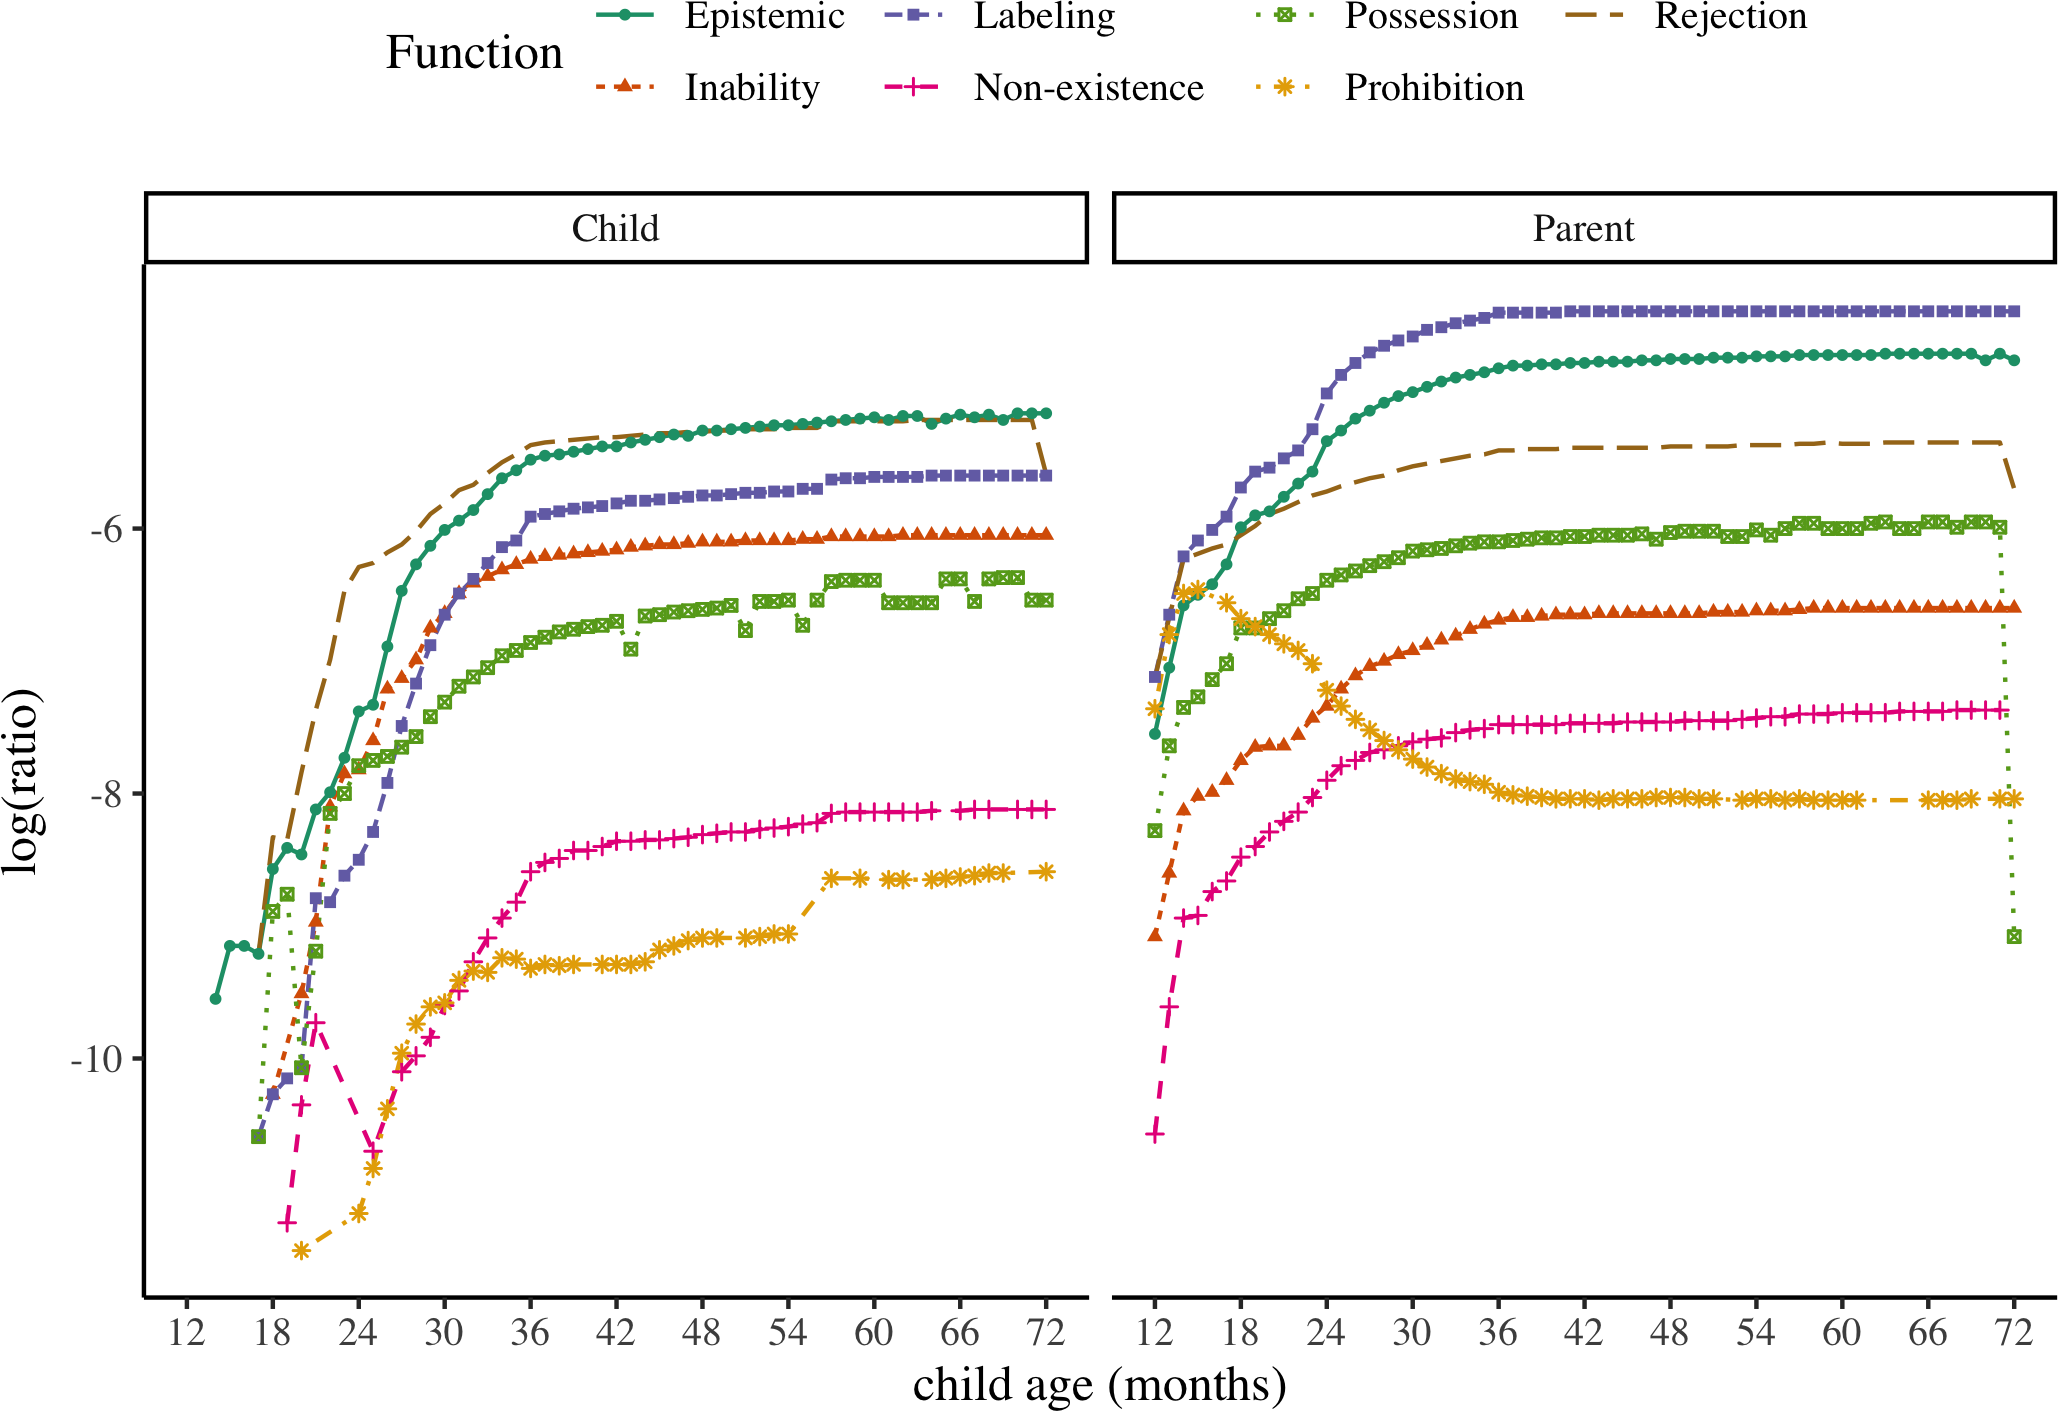
\includegraphics{neg_construction_article_files/figure-latex/allneg-1} 

}

\caption{Log cumulative ratios for all negative constructions at the syntactic level.}\label{fig:allneg}
\end{figure}

Figure \ref{fig:allpos} shows the log cumulative ratios of all positive counterparts to our negative constructions at the sentence level. Looking at parents productions on the right panel, we see that for almost all constructions, parents productions are stable and constant. Again, the only exception is positive prohibitions (imperatives). Parents produce positive prohibitions much more frequently at the beginning and between 12-36 months of child's age, but their production rates decrease later. This pattern mirrors what we see in Figure \ref{fig:allneg} with (negative) prohibitions, and suggests that parents use imperatives (positive or negative) with a higher frequency than ``normal'' at the beginning of children's development. Looking at children's positive productions on the left panel, we see that children start producing all positive counterparts to our negative constructions before 24 months of age. By 36 months, almost all positive constructions are being produced at a relatively constant rate close to parents' levels. An exception may be the epistemic construction which shows a gradual increase in frequency up until the 48-72 months (4-to-6 years) age period. Another noteworthy pattern is the relative high frequency of positive counterparts to prohibitions in the 12-24 months age period. Unlike (negative) prohibitions that were produced with some delay (compared to other constructions) around 24-30 months, positive imperatives are produced with high frequency even before 24 months of age. In other words, even though children do not frequently prohibit parents from doing things, they seem to be frequently ordering parents to do things for them; an observation that probably does not surprise any parent or caregiver!

\begin{figure}[H]

{\centering 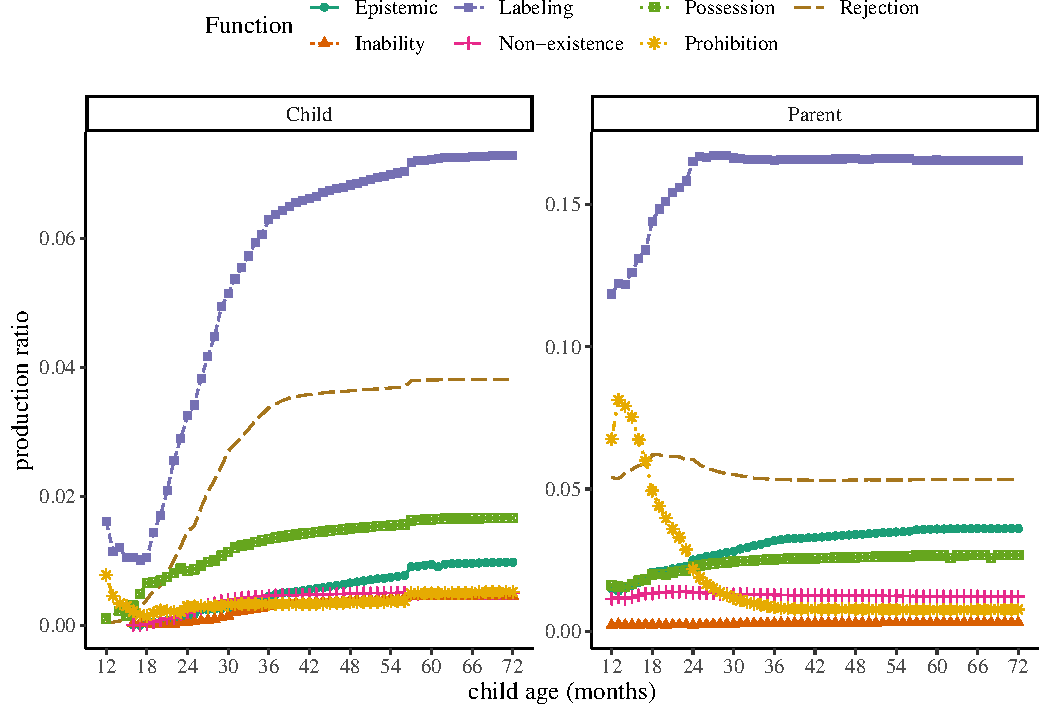
\includegraphics{neg_construction_article_files/figure-latex/allpos-1} 

}

\caption{Log cumulative ratios for the positive counpterparts to all negative constructions at the syntactic level.}\label{fig:allpos}
\end{figure}

Finally, Figure \ref{fig:alldiscourse} shows the log cumulative ratios of all negative responses to a previous utterance that used the negative constructions or their positive counterparts. Starting with parents' productions on the right, we see again a relatively constant rate of producing negative responses to each construction. The main exception is again prohibitions. Parents' start with very frequent ``\emph{no!}''-responses to imperatives produced by children, but the frequency of these negative responses drops to a relatively low and stable level after children are 36 months of age. Looking at children's negative responses on the left panel, we see that productions begin for all functions before 30 months of age and by 36 months children are already producing negative responses at a relatively constant rate close to parents production levels. The most striking difference between our discourse level and sentence level results are the frequency of rejection and labeling constructions. At the discourse level, parents' and children say \emph{no} to labeling and rejection much more frequently than other constructions, and they are produced earlier as well.

\begin{figure}[H]

{\centering 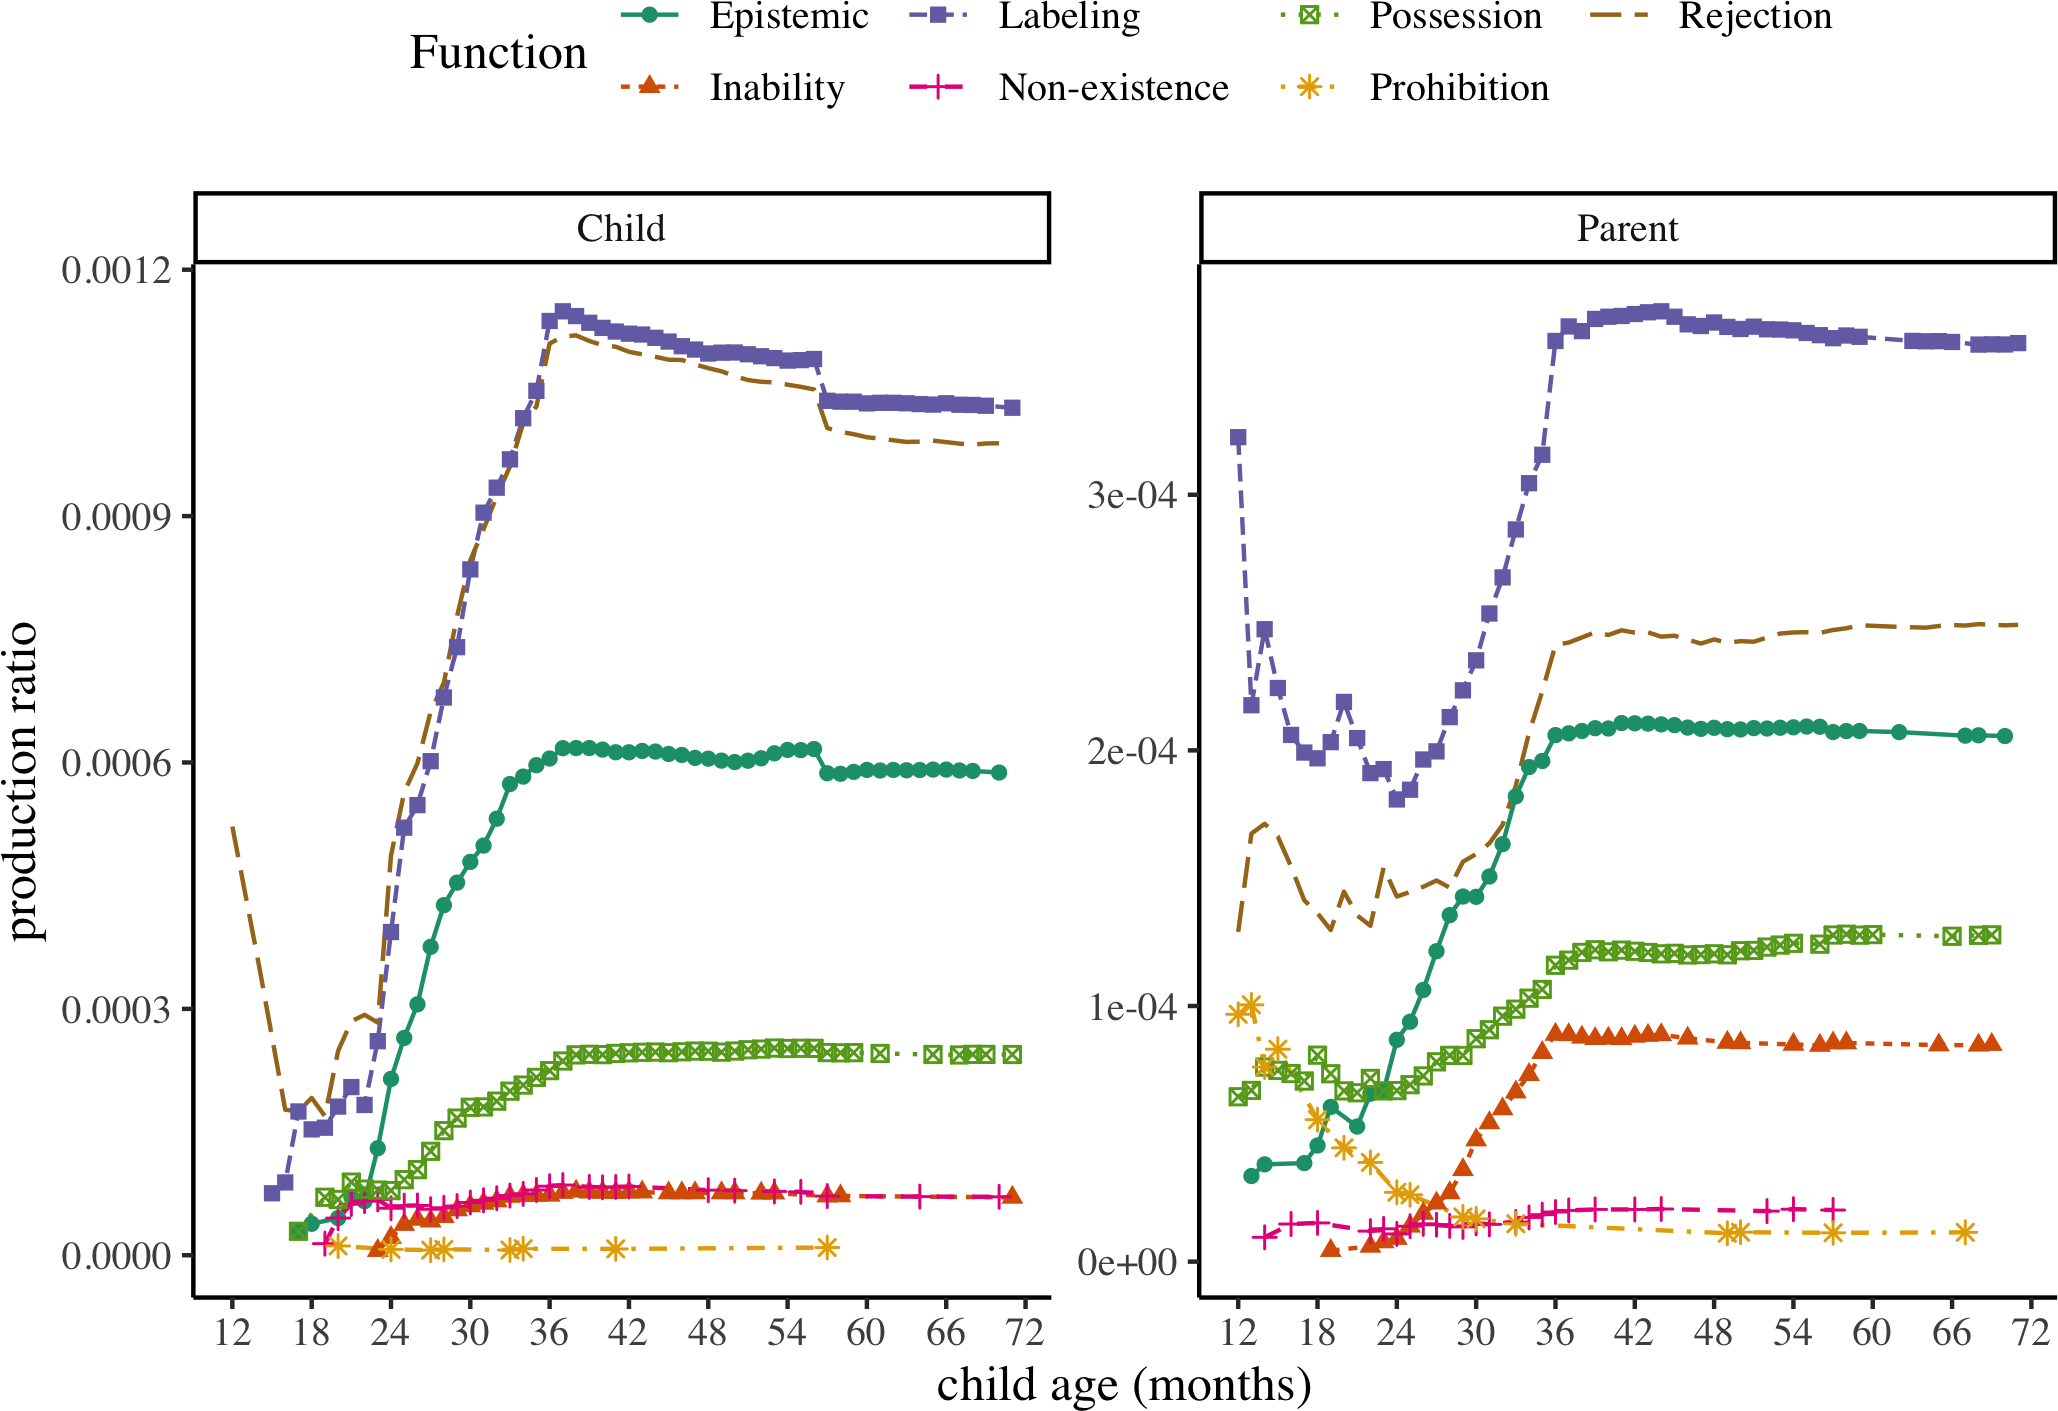
\includegraphics{neg_construction_article_files/figure-latex/alldiscourse-1} 

}

\caption{Cumulative ratios for all negative constructions at the discourse level.}\label{fig:alldiscourse}
\end{figure}

\hypertarget{conclusion}{%
\section{Conclusion}\label{conclusion}}

Using automatic annotations of large-scale corpora of child-parent interactions, we presented production trajectories for seven negative constructions that tend to express rejection, non-existence, prohibition, inability, labeling, epistemic states, and possession (Table 1). The results suggest that the production of almost all these negative constructions (except for prohibition) emerges and gradually increases within the 18-36 months age range (Figure 8). Their production frequencies remain stable and regular after 36 months and relatively close to parents' levels of production. It is important to note that similar to prior studies, our conclusions are limited to negation in children's production. Systematic experiments testing children's comprehension of negative utterances with different communicative functions are necessary to better understand the origins and developmental trajectory of negation.

A different hypothesis is that from the start, negation is an abstract concept that can serve different communicative functions. The main task of the learner is to break the speech stream, detect negative morphemes like \emph{no}, \emph{not}, or \emph{nt'}, and map them to this abstract meaning. She should then learn to use them appropriately in composition with other words to convey the right communicative function in context. There is either no substantial conceptual development for a logical concept such as negation, or this development is complete by the time the process of form-meaning mapping starts. This account predicts that conceptualy speaking, different communicative functions should be learnable and expressable early on and around the same time. Any delays in the comprehension or production of negative constructions and functions must be due to lack of experience with that construction or limitations in children's productive capacity. Therefore, it is possible for communicative functions of negation to not be comprehended or produced in fixed and ordered stages. Children may vary considerably on what constructions or functions they comprehend or produce earlier.

There are a few theoretical and methodological caveats, however. Studies that hypothesize stages in the development of negation almost exclusively study children's productions. Our methods of data collection and analysis may also affect our ability to provide data for or against these hypotheses.

Nevertheless, there seems to be some consensus among researchers that the crucial period for the development of negation is the period between 18 and 30 months of age. Some researchers suggest that by 36 months, children have an abstract concept of negation that is used to convey a variety of communicative functions (Cameron-Faulkner, Lieven, \& Theakston, 2007; McNeill \& McNeill, 1968; Pea, 1978).

Fourth, previous studies have almost exclusively focused on children's production of negation. A tacit assumption is that children's linguistic production provides a straightforward window into their conceptual development. However, children's linguistic comprehension may differ substantially from their production, and these in turn may differ from their conceptual representations. \ldots{} Therefore, developmental patterns

For future work, we would like to explore several directions. First, to more thoroughly examine and potentially model the developmental trajectories of negation in child production, certain production-specific factors (e.g.~length of utterance, ease of pronunciation) should be taken into account as well. In addition, we aim to investigate the production trajectory of positive counterparts to our negative structures (e.g.~``I know'' for ``I don't know''). Comparisons of negative utterances in relation to their positive counterparts would allow us to further analyze the developmental paths of negation within specific constructions.

Lastly, our experiments have concentrated on larger syntactic structures at the utterance level, hence cases where negation is used as discourse markers to respond to previous utterance(s) were excluded. However, these instances also have important semantic and conceptual roles in the communication between children and parents (e.g.~parent: \emph{do you want some bread?}; child: \emph{no no no}). Thus inclusions of negative structures at a more comprehensive level would be able to paint a more clear picture about the development of negation.

\begingroup
\setlength{\parindent}{-0.5in}
\setlength{\leftskip}{0.5in}

\endgroup

\hypertarget{refs}{}
\begin{CSLReferences}{1}{0}
\leavevmode\hypertarget{ref-diaparser}{}%
Attardi, G., Sartiano, D., \& Yu, Z. (n.d.). DiaParser attentive dependency parser. \emph{Submitted for Publication}.

\leavevmode\hypertarget{ref-bloom1970language}{}%
Bloom, L. M. (1970). \emph{Language development: Form and function in emerging grammars} (PhD thesis). Columbia University.

\leavevmode\hypertarget{ref-Brown1973}{}%
Brown, R. (1973). \emph{A first language, the early stages}. Cambrdige, Mass: Harvard University Press.

\leavevmode\hypertarget{ref-cameron2007part}{}%
Cameron-Faulkner, T., Lieven, E., \& Theakston, A. (2007). What part of no do children not understand? A usage-based account of multiword negation. \emph{Journal of Child Language}, \emph{34}(2), 251.

\leavevmode\hypertarget{ref-choi1988semantic}{}%
Choi, S. (1988). The semantic development of negation: A cross-linguistic longitudinal study. \emph{Journal of Child Language}, \emph{15}(3), 517--531.

\leavevmode\hypertarget{ref-darwin1872expression}{}%
Darwin, C. (1872). \emph{The expression of the emotions in man and animals}. John Murray.

\leavevmode\hypertarget{ref-demuth2006word}{}%
Demuth, K., Culbertson, J., \& Alter, J. (2006). Word-minimality, epenthesis and coda licensing in the early acquisition of {E}nglish. \emph{Language and Speech}, \emph{49}(2), 137--173.

\leavevmode\hypertarget{ref-macwhinney2000childes}{}%
MacWhinney, B. (2000). \emph{The CHILDES project: Tools for analyzing talk. Transcription format and programs} (Vol. 1). Psychology Press.

\leavevmode\hypertarget{ref-mcneill1968}{}%
McNeill, D., \& McNeill, N. (1968). What does a child mean when he says "no"? In E. M. Zale (Ed.), \emph{Studies of child language development} (pp. 51--62).

\leavevmode\hypertarget{ref-nordmeyer2018individual}{}%
Nordmeyer, A., \& Frank, M. C. (2018). Individual variation in children's early production of negation. In \emph{Proceedings of the 40th annual meeting of the cognitive science society} (pp. 2167--2172).

\leavevmode\hypertarget{ref-pea1978}{}%
Pea, R. (1978). \emph{The development of negation in early child language} (PhD thesis). University of Oxford.

\leavevmode\hypertarget{ref-qi-etal-2020-stanza}{}%
Qi, P., Zhang, Y., Zhang, Y., Bolton, J., \& Manning, C. D. (2020). {S}tanza: A python natural language processing toolkit for many human languages. In \emph{Proceedings of the 58th annual meeting of the association for computational linguistics: System demonstrations} (pp. 101--108). Online: Association for Computational Linguistics. \url{https://doi.org/10.18653/v1/2020.acl-demos.14}

\leavevmode\hypertarget{ref-sanchez2019childes}{}%
Sanchez, A., Meylan, S. C., Braginsky, M., MacDonald, K. E., Yurovsky, D., \& Frank, M. C. (2019). Childes-db: A flexible and reproducible interface to the child language data exchange system. \emph{Behavior Research Methods}, \emph{51}(4), 1928--1941.

\leavevmode\hypertarget{ref-dg}{}%
Tesnière, L. (1959). \emph{{É}l{é}ments de syntaxe structurale}. Paris: Klincksieck.

\leavevmode\hypertarget{ref-de1979form}{}%
Villiers, P. A. de, \& Villiers, J. G. de. (1979). Form and function in the development of sentence negation. \emph{Papers and Reports on Child Language Development}, \emph{17}, 57--64.

\leavevmode\hypertarget{ref-wei2006time}{}%
Wei, W. W. (2006). Time series analysis. In \emph{The oxford handbook of quantitative methods in psychology: Vol. 2}.

\end{CSLReferences}


\end{document}
